\documentclass[11pt]{article}

\usepackage[T1]{fontenc}
\usepackage[utf8]{inputenc}
\usepackage{lmodern}
\usepackage{microtype}

\usepackage{arxiv}

\usepackage{amsmath}
\usepackage{amssymb}
\usepackage{amsthm}
\usepackage{booktabs}
\usepackage{graphicx}
\usepackage{algorithm}
% `noend`: one-line bodies dominate here, and an explicit terminator after each
% of them costs more clarity than it buys. Indentation carries the structure.
\usepackage[noend]{algpseudocode}
\usepackage{tikz}
\usetikzlibrary{arrows.meta, positioning, fit, backgrounds, calc, patterns}
\usepackage{xcolor}
\usepackage[numbers,sort&compress]{natbib}
% Bibliography URLs are long enough to leave an underfull line if they can only
% break at punctuation; xurl lets them break anywhere.
\usepackage[hidelinks]{hyperref}
\usepackage{xurl}
\usepackage[capitalise,noabbrev]{cleveref}

% Each environment gets its own counter. Sharing one makes cleveref name every
% reference after the counter, so \cref of a definition comes out as "Theorem".
\theoremstyle{plain}
\newtheorem{theorem}{Theorem}
\newtheorem{proposition}{Proposition}
\theoremstyle{definition}
\newtheorem{definition}{Definition}
\theoremstyle{remark}
\newtheorem{remark}{Remark}

% The palette the figures were drawn with, so a TikZ schematic sitting beside
% one of them does not look like it came from a different document.
\definecolor{sccdTeal}{HTML}{0E8AA0}
\definecolor{sccdAmber}{HTML}{C07C10}
\definecolor{sccdPlum}{HTML}{8A3C74}
\definecolor{sccdMoss}{HTML}{3E6E4B}
\definecolor{sccdInk}{HTML}{333A41}
\definecolor{sccdGrid}{HTML}{D6DBE0}

% Notation used throughout, defined once.
\newcommand{\Fdiff}{\mathbf{F}}          % the difference function
\newcommand{\Rthree}{\mathbb{R}^{3}}
\newcommand{\toi}{t^{\star}}             % the reported time of impact
\newcommand{\toitrue}{\bar{t}}           % the true earliest root
\newcommand{\mach}{\varepsilon}          % machine epsilon
\newcommand{\dom}{\mathcal{B}}           % a box in (t, u, v)
\newcommand{\Cand}{\mathcal{C}}          % the candidate set
\newcommand{\Boxes}{\mathcal{B}}
\DeclareMathOperator{\hull}{hull}
% Small caps for the algorithm's named steps. Wrapped in \textnormal so it
% survives the italic body of a theorem, where lmodern has no italic small caps.
% The two primitives of a query, coloured as they are in the schematics: the
% teal and plum boxes of Figure 8 are the same two primitives whose difference
% function these equations root, so a reader can carry one picture into the
% other. Named by role rather than by colour, so the palette can change in one
% place.
\newcommand{\primA}[1]{\textcolor{sccdTeal}{#1}}
\newcommand{\primB}[1]{\textcolor{sccdPlum}{#1}}
% The quantity under test -- amber in both schematics, where it marks the query
% box, the overlap it forms, and the query that overruns a block.
\newcommand{\tested}[1]{\textcolor{sccdAmber}{#1}}

\newcommand{\op}[1]{\textnormal{\textsc{#1}}}

% Generated tables are as wide as their data. This shrinks one only when it
% would otherwise run into the margin, and leaves every table that already fits
% at its natural size -- so the common case keeps the body font exactly.
\newcommand{\fittable}[1]{%
  \resizebox{\ifdim\width>\linewidth \linewidth\else \width\fi}{!}{#1}}

\headertitle{Conservative continuous collision detection on CPU and GPU}
\preprintmark{\textsc{Preprint}}

\title{A Conservative Continuous Collision Detection Pipeline\\
       for Triangle and Quad Meshes on CPU and GPU}

% Affiliation marks run in order of first appearance, so Victoria is 3 rather
% than 7: it is Patrick's third and Teseo's only one, and the two share the entry.
\author{%
  Patrick Zulian\affilmark{1,2,3}\thanks{Corresponding author:
  \texttt{patrick.zulian@usi.ch}, ORCID 0000-0002-5822-3288.}
  \and David Belgrod\affilmark{4}
  \and Bolun Wang\affilmark{5}
  \and Zachary Ferguson\affilmark{6}
  \and Xin Zhao\affilmark{4}
  \and Marco Attene\affilmark{7}
  \and Daniele Panozzo\affilmark{4}
  \and Teseo Schneider\affilmark{3}%
}

\affiliations{%
  \affiltext{1}{Euler Institute, Universit\`a della Svizzera italiana,
    Via Buffi 13, 6900 Lugano, Ticino, Switzerland}
  \affiltext{2}{UniDistance Suisse, Schinerstrasse 18, 3900 Brig, Valais,
    Switzerland}
  \affiltext{3}{University of Victoria, Victoria, BC, Canada}
  \affiltext{4}{New York University, New York, NY, USA}
  \affiltext{5}{King Abdullah University of Science and Technology, Thuwal,
    Saudi Arabia}
  \affiltext{6}{Massachusetts Institute of Technology, Cambridge, MA, USA}
  \affiltext{7}{IMATI -- CNR, Genoa, Italy}%
}

\date{\today}

\begin{document}
\maketitle

\begin{abstract}
Continuous collision detection (CCD) determines whether two meshes moving along
linear trajectories touch during a time step, and at what time. A simulator that
guarantees an intersection-free state can tolerate neither a missed collision
nor a late time of impact, since both allow the solver to step through the
contact. We present SCCD, a CCD pipeline for triangle and quad meshes that is
conservative by construction on both CPU and GPU, and we assess it against the
certified reference implementation TightInclusion over $11{,}630{,}064$ checks
against exactly known roots.

The broad phase is a two-dimensional cell list requiring neither a sort nor a
user-chosen cell size, with one query per pair type: the vertex-face query bins
each box into every cell it touches, while the edge-edge query, being one list
against itself, binds each box to the single cell holding its minimum corner and
walks forward from it. The host narrow phase packs SIMD lanes with boxes drawn
from \emph{different} queries, which an order-independence argument shows to be
legal. The device narrow phase pairs a small per-block stack with a
double-buffered global queue, so that a query requiring millions of boxes
spreads across the machine.

Over six scenes and $6{,}394$ cases on one \textsc{GH200} node, SCCD reports no
missed collision and no late time of impact. On the host, the median and
worst-case error match TightInclusion's on all twelve scene-phases to every
printed digit, at $1.7\times$ to $4.9\times$ its speed. The device is
$2.5\times$ to $26.6\times$ faster and agrees to within $0.6\%$ and $4.5\%$. Its
narrow phase nevertheless runs at $0.56\times$ host speed on the smallest scene,
which places the whole pipeline behind the host there.
\end{abstract}


\keywords{continuous collision detection \and conservative algorithms \and
  interval methods \and GPU computing \and SIMD \and contact simulation}

\section{Introduction}
\label{sec:intro}

Continuous collision detection (CCD) asks a question that sounds simple and is
not. Take two configurations of a mesh, one at the start of a time step and one
at the end, with every vertex moving along a straight line in between. Does any
pair of primitives touch during the step, and if so, when? The answer gates the
step size in cloth, deformable and rigid-body simulation. The two ways of
getting it wrong are not symmetric.

If a method reports a collision that does not happen, the solver takes a shorter
step than it needed to. Work is wasted and nothing is broken. If a method misses
a collision, or reports a time of impact \emph{after} the true one, the solver
steps straight through the contact, and the configuration it lands in contains
an interpenetration. One family of solvers is built on a barrier
potential~\citep{li2020ipc,li2021codim,ferguson2021rigid}, and its whole
argument depends on the state remaining intersection-free. For those solvers the
result is worse than degraded: the barrier is infinite on the wrong side, and
the optimisation has nowhere to go.

\begin{definition}[Conservative]
\label{def:conservative}
A CCD implementation is \emph{conservative} if it reports a collision whenever
the geometries intersect during the step, and the time of impact it reports is
at or before the true earliest one.
\end{definition}

\Cref{def:conservative} is the specification this work implements, and it is
deliberately stronger than the usual one. Reporting the Boolean correctly is not
enough. A query can agree with an exact reference on whether a contact happens
and still return a time after it, which costs the solver as much as a missed
collision does. Every accuracy measurement in this paper is therefore
\emph{signed}, and a time of impact later than the exact root counts as a
failure of the same severity as a miss.

The difficulty is that conservativeness is a statement about real arithmetic,
while implementations run in floating point. \citet{wang2021tight} showed that
most published CCD implementations are not conservative once the rounding is
accounted for, and they gave the first one that provably is. That
implementation, TightInclusion, replaces interval arithmetic with a custom
inclusion function and a certified error bound. It is the reference we measure
against throughout, used exactly as released.

\paragraph{This work.} We present SCCD, a two-phase CCD pipeline for triangle
\emph{and} quad meshes, with host and device implementations of both phases. Its
conservativeness is structural and not empirical (\cref{sec:guarantee}), and we
assess it against TightInclusion on a dataset whose roots are known exactly. The
contribution is the parallel design, its measured performance and the accuracy
assessment, and not an implementation of a known algorithm on new hardware.

The first contribution is a broad phase with no tuning parameter and no sort: a
two-dimensional uniform cell list whose cell size comes from the data itself.
Its two queries have different shapes and are built differently. Vertex-face
bins a box into every cell its extent touches and attributes a pair to the cell
holding the corner of the overlap (\cref{sec:bp:cell}). Edge-edge is one list
against itself, which admits one entry per box at its minimum corner and a
forward walk in row-major cell order, pruned by a prefix maximum per row of
cells, so no bound on how many cells a box may span is needed
(\cref{sec:bp:self}).

The second is a host narrow phase that packs single-instruction,
multiple-data (SIMD) lanes across queries. TightInclusion's search is a
priority queue ordered by the time lower bound, and its answer is the first box
it accepts. We show in \cref{sec:np:order} that keeping the minimum over
\emph{all} accepted boxes and pruning against it gives the same answer under
\emph{any} traversal order. That licenses a lane to hold boxes from different
queries (\cref{alg:host}), which turns a search with per-query divergence into
a vector kernel. Sibling boxes then inherit four of their eight corner values
from their parent, halving the dominant cost.

The third is a device narrow phase built around redistribution. The difficulty of a CCD query is heavy-tailed: on one scene most
queries need a single box, while $208$ of them need more than a million
(\cref{tab:difficulty}). A large per-block work stack keeps such a query inside
the block that seeded it while its neighbours idle. We use a deliberately
\emph{small} shared stack that spills early into a double-buffered global
queue, which the next launch redistributes across every block
(\cref{alg:device}). On the worst scene this is worth two orders of magnitude
(\cref{tab:stackcap}).

The fourth is a signed accuracy assessment against a certified reference. It
covers $11{,}630{,}064$ query-mode checks against exact symbolic roots, on both
processors and all six scenes, of which $11{,}044{,}766$ place a reported time
of impact beside an exact root. SCCD reports no missed collision and no late
time of impact, and reproduces TightInclusion's median and worst-case error to
every printed digit while running faster (\cref{sec:results:ref}).

We are equally explicit about where the pipeline does not win, and why. The device narrow phase is slower than the host on four of six scenes, for a
structural reason we can name, and that is enough to put the whole pipeline
behind on one of them. The host cell list beats the device broad phase at every
mesh size we measured, and by more as the mesh grows. The mode that trades accuracy for speed is \emph{slower} on
half the host scenes. \Cref{sec:limitations} collects those results, together
with the threats to validity that bound what the measurements can support.

\subsection{Prior work}
\label{sec:related}

CCD is conventionally split into two stages. A \emph{broad phase} is a
conservative filter: it discards pairs of primitives whose swept bounding
volumes cannot meet. A \emph{narrow phase} then decides each surviving pair
precisely enough to be trusted. The two stages have separate literatures and
separate failure modes.

\subsubsection{Broad phase}

Broad phases fall into three families: sweep and
prune~\citep{baraff1992dynamic,cohen1995icollide}, with numerous parallel and
incremental
variants~\citep{capannini2018adaptive,tracy2009sweep,liu2010realtime}; uniform
grids and spatial hashes~\citep{tang2018icloth,tang2018pscc}; and hierarchies of
bounding volumes, KD-trees and interval
trees~\citep{serpa2019kdtree,serpa2020broadmark,zomorodian2000boxes}, which
prune better per test and are harder to build and traverse in parallel.

Grids parallelise well and need no sort, and they introduce a parameter, the
cell size, which the literature repeatedly identifies as the method's weak
point: a cell that is too small lets duplicate candidates exhaust memory, one
that is too large degenerates towards brute force, and no single value serves a
scene whose geometry changes over the simulation. \Cref{sec:bp:cell} derives the
cell from the swept boxes themselves and caps the cell count relative to the
element count, so no value is left for a user to choose. These methods also have to suppress the pairs a box meets in more
than one cell, whether by a rule on the cell or by a pass over the output.
\Cref{sec:bp:grid} gives a box one cell instead, the arrangement linked-cell
neighbour search uses~\citep{allen2017liquids}, which requires the cells to
carry an order and a bound and requires no test on the pairs.

\silentoverflow. Our broad
phase bins the boxes, so it inherits neither the sort's cost nor its dependence
on one axis separating the geometry.

\subsubsection{Narrow phase}

For linear trajectories and no minimum separation, a vertex-face or edge-edge
query reduces to finding roots of a cubic. Numerical cubic
solving~\citep{provot1997collision,bridson2002robust} assumes exact arithmetic
and in floating point both misses collisions and invents them. Conservative
advancement~\citep{mirtich1996impulse,tang2010local,lan2022penetration} advances
time by repeated minimum-distance queries, which involve square roots, so the
underestimate it relies on is not certified. Of the exact methods, root-parity
tests~\citep{brochu2012efficient,tang2014bernstein,wang2022rootparity} cannot
distinguish zero roots from two; symbolic root finding is genuinely exact, takes
seconds per query, and produced the ground truth used in this paper.

\emph{Inclusion-based} root finding is the family this work belongs to. These
methods evaluate an inclusion function over a box in parameter space, discard
the box when the function's range provably excludes the origin, and otherwise
refine~\citep{snyder1992interval,snyder1993interval,vonherzen1990geometric}.
Interval arithmetic~\citep{moore2009interval} gives such a bracket and
overestimates it. \citet{wang2021tight} construct an inclusion function specific
to these queries together with a forward error bound; theirs is the first
implementation whose conservativeness survives the implementation, and
TightInclusion is that implementation. \citet{belgrod2025toi} restructure the
same mathematics for a GPU, and \citet{li2021codim} take the additive route
instead. Both are measured in \cref{sec:results:others}.

SCCD inherits TightInclusion's mathematics. It uses the same inclusion function
in the same expression order, the same certified bound and the same acceptance
conditions, and it differs only in how the search is realised on each processor.
\Cref{sec:np:order} gives the argument that licenses the difference, and
\cref{sec:parallel} gives the two realisations. We do not consider a search that
is part this one and part the reference: such a hybrid inherits the certificate
of neither, and the reference itself serves a caller who wants the reference's
answer.

\section{Problem statement and the inclusion function}
\label{sec:prelim}

The collision queries treated here reduce to finding roots of a map $\Fdiff$ on
a three-dimensional parameter box, and that map is multilinear. Multilinearity
means that the eight corner values of a box give the \emph{exact} range of
$\Fdiff$ over it, which in real arithmetic would settle the matter. In floating
point the corner values are perturbed, and a certified bound on the perturbation
is what stands between the search and an unsound answer. This section sets out
both properties, together with the tolerances that tell the search when to stop.
\Cref{sec:guarantee} turns them into a guarantee, and \cref{sec:parallel} into
two implementations.

\subsection{The queries and their difference function}
\label{sec:prelim:queries}

A mesh is given at two instants. Vertex $p$ is at $p^{0}$ at time $t=0$ and at
$p^{1}$ at $t=1$, and moves affinely in between, $p(t) = (1-t)\,p^{0} +
t\,p^{1}$. Two triangle meshes intersect during the step if and only if a vertex
passes through a face or an edge crosses an edge~\citep{provot1997collision}, so
the whole problem reduces to two elementary queries, each expressed as a root of
a map $\Fdiff : [0,1]^{3} \to \Rthree$.

For a \emph{vertex-face} query with vertex $\primA{q}$ and face
$(\primB{f_{1}},\primB{f_{2}},\primB{f_{3}})$, writing $o = 1-u-v$ for the third
barycentric coordinate,
\begin{equation}
\label{eq:fvf}
\Fdiff(t,u,v) \;=\; \primA{q(t)} \;-\; \primB{\bigl[\,o\,f_{1}(t) + u\,f_{2}(t)
+ v\,f_{3}(t)\,\bigr]}, \qquad (u,v)\in\Delta,
\end{equation}
where $\Delta = \{(u,v) : u,v \ge 0,\ u+v \le 1\}$. For an \emph{edge-edge}
query with edges $(\primA{a_{0}},\primA{a_{1}})$ and
$(\primB{b_{0}},\primB{b_{1}})$,
\begin{equation}
\label{eq:fee}
\Fdiff(t,u,v) \;=\; \primA{\bigl[a_{0}(t) + u\,(a_{1}(t)-a_{0}(t))\bigr]} \;-\;
\primB{\bigl[b_{0}(t) + v\,(b_{1}(t)-b_{0}(t))\bigr]}, \qquad (u,v)\in[0,1]^{2}.
\end{equation}
A contact occurs exactly when $\Fdiff$ vanishes somewhere on the domain, and the
earliest time of impact is $\toitrue = \min\{\,t : \Fdiff(t,u,v)=0 \text{ for
some admissible } (u,v)\,\}$.

Quad meshes add a third query of the same shape. For a vertex against a
bilinear quad with corner nodes $\primB{g_{1}},\dots,\primB{g_{4}}$,
\begin{equation}
\label{eq:fvq}
\Fdiff(t,u,v) \;=\; \primA{q(t)} \;-\; \primB{\sum_{k=1}^{4} w_{k}(u,v)\,
g_{k}(t)}, \qquad
w = \bigl((1-u)(1-v),\; u(1-v),\; (1-u)v,\; uv\bigr),
\end{equation}
on $(u,v)\in[0,1]^{2}$. The weights in \cref{eq:fvq} put the nodes in
\emph{lexicographic} order, the corners $(0,0)$, $(1,0)$, $(0,1)$ and $(1,1)$ of
the parameter square, and not the cyclic winding a quad is usually stored with.
\Cref{sec:np:quad} quantifies the cost of an incorrect ordering.

The three queries share the property that the search exploits. Each of
\cref{eq:fvf,eq:fee,eq:fvq} is \emph{multilinear}: affine in $t$ for fixed
$(u,v)$, affine in $u$ for fixed $(t,v)$, and affine in $v$ for fixed $(t,u)$.
On an axis-aligned box $\dom =
[t_{\ell},t_{h}]\times[u_{\ell},u_{h}]\times[v_{\ell},v_{h}]$ a multilinear map
attains its extrema at vertices of the box, so for each component $d$,
\begin{equation}
\label{eq:hull}
\Fdiff_{d}(\dom) \;=\; \bigl[\;\min_{c \in V(\dom)} \Fdiff_{d}(c),\;
\max_{c \in V(\dom)} \Fdiff_{d}(c)\;\bigr],
\end{equation}
where $V(\dom)$ are the eight corners. \Cref{eq:hull} is an equality and not an
enclosure: evaluating the eight corners and taking the componentwise hull gives
the exact range of $\Fdiff$ over $\dom$. That property distinguishes the
inclusion function of \citet{wang2021tight} from generic interval arithmetic,
which widens at every operation, and it allows a box to be discarded on the
strength of its corners alone.

\subsection{Error bound and the tolerances}
\label{sec:prelim:err}

The exactness of \cref{eq:hull} is a statement about real arithmetic, whereas
the eight values a machine computes are $\Fdiff_{d}(c)$ perturbed by rounding.
Since \cref{eq:hull} is the only thing licensing a box to be discarded, the size
of that perturbation is the only thing standing between the search and a lost
root.

\citet{wang2021tight} bound it by a forward error analysis in the standard
style~\citep{higham2002accuracy}, the same reasoning that underlies the
floating-point filters used for exact geometric
predicates~\citep{attene2020indirect}. With $\mach$ the unit roundoff and $M$
the largest absolute coordinate appearing among the eight input points of the
query,
\begin{equation}
\label{eq:err}
\delta \;=\; \min(M,\,1),
\qquad
\epsilon_{d} \;=\; \kappa\,\mach\,\delta^{3},
\qquad
\kappa = \begin{cases}
30 & \text{vertex-face},\\
28 & \text{edge-edge},
\end{cases}
\end{equation}
and every computed corner value lies within $\epsilon_{d}$ of the exact one.

Two details of \cref{eq:err} are essential. The first is that $\delta$ is $M$
clamped from \emph{above} by $1$. Clamping from below instead would make the pad
grow as the cube of the scene's diameter, reaching $10^{6}$ at a scale of $100$,
which the acceptance test would then have to spend.

The second is that the bound is derived for one particular sequence of
floating-point operations. An algebraically identical but differently associated
expression has a different rounding profile, and $\kappa$ does not cover it. The
corner evaluation is therefore written in TightInclusion's order and is not free
to be rearranged. The implementation pins IEEE semantics across those regions,
and no \texttt{-ffast-math} compilation flag is used anywhere in this work.

No constant is certified in the literature for the bilinear query of
\cref{eq:fvq}. We use $\kappa = 38$, which exceeds both certified constants and
is therefore safe in the direction that matters, and we record it as an
over-estimate; lowering it requires a derivation.

The bound determines when a box may be discarded, and a second quantity
determines when a box is small enough for refinement to stop. That quantity is
measured per axis, since the three axes of the domain are not commensurate: a
width in $t$ and a width in $u$ mean different things. Following
\citet{wang2021tight}, a user-facing distance tolerance $\tau$ in the codomain
becomes per-axis domain tolerances by division by the rate at which $\Fdiff$
changes along each axis,
\begin{equation}
\label{eq:tol}
\tau_{0} = \frac{\tau}{L_{t}},\qquad
\tau_{1} = \frac{\tau}{L_{u}},\qquad
\tau_{2} = \frac{\tau}{L_{v}},
\end{equation}
with each $L$ the largest $\ell_{\infty}$ displacement of the relevant corner
differences along that axis.

\Cref{eq:tol} requires a cap. A query whose geometry barely moves along one axis
divides by nearly zero and receives an effectively infinite tolerance, so that
every box satisfies ``width $\le$ tolerance'', the root box is accepted on
sight, and the query reports $\toi = 0$. That outcome is conservative, being
early and not late, and it is also uninformative. The quotients are therefore
clamped at $\tau_{0}\le 10^{-3}$ and $\tau_{1},\tau_{2}\le 10^{-2}$, matching
the reference. The same two caps are compiled into the device kernels, so both
processors stop in the same place.

Together, \cref{eq:hull,eq:err,eq:tol} fix what an implementation of this family
can promise. Exactness is not attainable at simulation speed, whereas
conservativeness in the sense of \cref{def:conservative} is, at the price of
false positives, which \cref{sec:results} reports per scene as the cost they
are.

Deciding a query costs far more than deciding whether it is worth asking, so the
pipeline applies the cheaper test first. \Cref{sec:bp} describes that filter,
which needs none of the machinery above, and \cref{sec:np} the search that uses
all of it.

\section{Broad phase}
\label{sec:bp}

Of the two phases the broad one asks the cheaper question. It never evaluates
$\Fdiff$ and never sees a tolerance. It turns a mesh into a set of candidate
pairs, meaning pairs of primitives whose swept bounding boxes overlap and which
might therefore touch, and hands them to \cref{sec:np}. It must be
conservative, because a pair it discards is never examined again. On the scenes
in our benchmark it is also the larger share of the host runtime, so it must be
fast.

One algorithm serves it, over one acceleration structure: a uniform grid on two
of the three axes. The two queries it answers are not the same shape, so they
are described separately. Vertex-face asks one list against another and is
answered by binning a box into every cell its extent touches
(\cref{sec:bp:cell}); edge-edge asks one list against itself, which admits a
cheaper binning and a different walk (\cref{sec:bp:self}).

\subsection{Swept boxes, and the shape of the output}
\label{sec:bp:common}

Because vertices move affinely, the axis-aligned box enclosing a primitive's
entire trajectory is the componentwise hull of its vertex positions at $t=0$ and
$t=1$. That hull is exact and needs no sampling. One box is built per vertex,
per edge and per face. Where the box is stored in a narrower type than the
geometry, each bound is moved outward by one unit in the last place, so a
rounded box can never exclude a candidate the exact box would have kept.

Two conventions shape everything downstream. The first concerns the overlap
test, which rejects only on a \emph{strict} separation, $a_{\min} > b_{\max}$ on
some axis. Boxes that merely touch are therefore reported as overlapping. This
inclusivity is deliberate: a candidate window that rejects a pair of boxes
merely touching drops the pairs a moving surface produces most often, which are
the degenerate ones.

The second is that all storage is structure-of-arrays and every output is built
\emph{count-then-fill}. A first pass counts the pairs each primitive will
contribute, a prefix sum turns those counts into offsets, and a second pass
re-runs the identical traversal, writing into its own slice. Nothing grows a
shared buffer, the allocation is exact, and the output is bit-for-bit
reproducible. The same code shape then works on a GPU, where a growable
per-thread container is not available.

The host tests one box against $32$ consecutive boxes at a time, and an AVX-512,
AVX2 or NEON kernel returns a $32$-bit mask of the survivors. Counting is then a
population count, and enumeration is a bit scan. A rejected candidate therefore
never issues the indirect load of its element indices, which is the expensive
part of a test that usually fails.

\subsection{The vertex-face query}
\label{sec:bp:cell}

Vertex-face takes two lists, the faces against the vertices, and
\cref{alg:cell} answers it by binning one of them into a grid. Two of its
choices are deliberate enough to state before the algorithm itself.

The grid is over \emph{two} axes, not three. For a surface of $N$ elements of
size $h$ inside a region of side $L$ we have $N \sim (L/h)^{2}$, because a
surface does not fill a volume. A two-dimensional grid at element resolution
therefore has $O(N)$ cells, and it is mostly occupied. A three-dimensional one
has $(L/h)^{3} = N^{3/2}$ cells. At $N = 1.5\times10^{6}$ that is
$1.8\times10^{9}$ cells at $0.08\%$ occupancy, which buys memory and empty-cell
iteration in exchange for pruning along a direction the surface barely occupies.
The third axis is not abandoned. The ordinary three-dimensional box test inside
the cell culls it, where it costs nothing extra.

The cell size is derived, not chosen. The grid spacing on each of the two axes
is the \emph{mean extent of the swept boxes} on that axis. The resulting cell
counts are then scaled isotropically so that their product does not exceed $4N$:
past that point more resolution does not pay, and a degenerate extent could
otherwise allocate without bound. No voxel size is left for a caller to supply,
and none to get wrong.

Two other spacings suggest themselves and both are worse, for opposite reasons.
Sizing on the \emph{element} size makes the grid far too fine: a swept box is
much larger than the element it came from, so every box would span a block of
cells and the binning pass would cost more than the query saves. Sizing on the
\emph{largest} box is the textbook uniform-grid rule, and it is the more
tempting of the two, because it buys a property the mean does not -- if no box
is wider than a cell, then two overlapping boxes lie within one cell of each
other and a fixed $3\times3$ stencil around a single owning cell finds every
partner, with no duplicates to settle. What that rule costs is that the widest
box in the scene sets the spacing for all of them. The swept boxes are not of
one size: the widest is $4.5\times$ the mean on armadillo-rollers' vertices and
$24\times$ on cloth-funnel's edges, because a few elements move fast while most
barely move. On armadillo-rollers one swept edge spans $11\%$ of the scene, so a
cell at least that wide admits an $8\times9$ grid at any element count, and the
scene's $36{,}363$ edges land in $72$ cells, $505$ to a cell. Measured, that
costs the host broad phase up to $11.9\times$. The mean keeps the cost of a box
proportional to that box's own size, which is what a heavy-tailed size
distribution requires.

\begin{algorithm}[htbp]
\caption{The vertex-face query, one pass (count or fill)}
\label{alg:cell}
\begin{algorithmic}[1]
\Function{CellList}{$A$, $B$}
  \State $(a_{0},a_{1}) \gets$ the two axes of largest centre variance
  \State $h_{k} \gets$ mean extent of the boxes on axis $a_{k}$;\quad
         $n_{k} \gets \lfloor \operatorname{span}_{k}/h_{k} \rfloor$,
         scaled so $n_{0}n_{1} \le 4N$
  \State count the cells of each box of $B$, prefix-sum them, and scatter
         each box index into its cells
  \ForAll{$i$ \textbf{in parallel}}
    \ForAll{cells $c$ touched by $A_{i}$, and $j$ listed in $c$}
      \If{$A_{i}$ and $B_{j}$ are disjoint in 3D} \textbf{continue} \EndIf
      \State $o_{k} \gets \max(A_{i}.\min_{a_{k}},\, B_{j}.\min_{a_{k}})$
        \Comment{corner of the overlap}
      \If{$c \ne \operatorname{cell}(o_{0},o_{1})$} \textbf{continue}
        \Comment{another cell owns this pair}
      \EndIf
      \If{$A_{i}$ and $B_{j}$ share a vertex} \textbf{continue} \EndIf
      \State count, or emit the pair
    \EndFor
  \EndFor
\EndFunction
\end{algorithmic}
\end{algorithm}

\begin{figure}[htbp]
  \centering
  % The cell list in detail: (a) how the structure is built, (b) how a pair met
% in several cells is emitted once.
%
% No prose inside the drawing. What the panels mean belongs in the caption,
% where it can be read at caption size and does not compete with the marks.
%
% Grids are drawn line by line rather than with TikZ's `grid`, which places its
% lines at multiples of the step measured from the origin and not from the
% corner of the rectangle given to it.
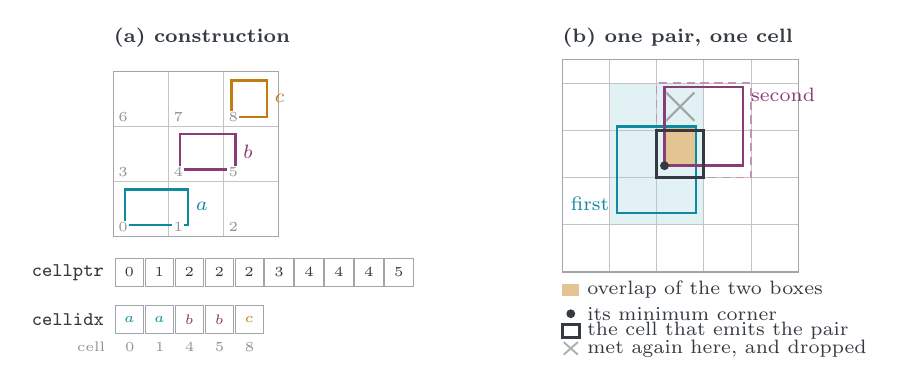
\begin{tikzpicture}[
  font=\scriptsize,
  >={Stealth[length=1.6mm]},
  lbl/.style={font=\scriptsize, text=sccdInk, inner sep=1.5pt},
  tiny/.style={font=\tiny, text=sccdInk, inner sep=1pt},
  ttl/.style={font=\scriptsize\bfseries, text=sccdInk, inner sep=0pt},
  slot/.style={draw=sccdInk!45, line width=0.3pt, minimum width=3.6mm,
               minimum height=3.6mm, inner sep=0pt, font=\tiny, text=sccdInk},
  lead/.style={draw=sccdInk!55, line width=0.3pt},
]

% ============================== (a) construction =============================
% Three boxes over a 3x3 grid, and the two arrays they bin into. Cells are
% numbered row-major from the bottom left, which is the order cell_of gives.
\begin{scope}
  \node[ttl, anchor=south west] at (0,3.30) {(a) construction};

  \foreach \x in {0,0.70,1.40,2.10}
    \draw[draw=sccdInk!30, line width=0.3pt] (\x,0.90) -- (\x,3.00);
  \foreach \y in {0.90,1.60,2.30,3.00}
    \draw[draw=sccdInk!30, line width=0.3pt] (0,\y) -- (2.10,\y);
  \draw[draw=sccdInk!45, line width=0.4pt] (0,0.90) rectangle (2.10,3.00);

  \draw[draw=sccdTeal, line width=0.9pt] (0.15,1.05) rectangle (0.95,1.50);
  \draw[draw=sccdPlum, line width=0.9pt] (0.85,1.75) rectangle (1.55,2.20);
  \draw[draw=sccdAmber, line width=0.9pt] (1.50,2.42) rectangle (1.95,2.88);
  \node[lbl, text=sccdTeal, anchor=west] at (0.99,1.28) {$a$};
  \node[lbl, text=sccdPlum, anchor=west] at (1.59,1.98) {$b$};
  \node[lbl, text=sccdAmber, anchor=west] at (1.99,2.65) {$c$};

  % The cell numbers go on last, so a box cannot hide one.
  \foreach \c/\cx/\cy in {0/0.04/0.94, 1/0.74/0.94, 2/1.44/0.94,
                          3/0.04/1.64, 4/0.74/1.64, 5/1.44/1.64,
                          6/0.04/2.34, 7/0.74/2.34, 8/1.44/2.34}
    \node[tiny, text=sccdInk!55, anchor=south west, fill=white,
          inner sep=0.5pt] at (\cx,\cy) {\c};

  % --- the two arrays ---
  \node[lbl, anchor=east] at (-0.06,0.44) {\texttt{cellptr}};
  \foreach \i/\v in {0/0, 1/1, 2/2, 3/2, 4/2, 5/3, 6/4, 7/4, 8/4, 9/5}
    \node[slot, anchor=south west] at ({0.02 + \i*0.38},0.26) {\v};

  \node[lbl, anchor=east] at (-0.06,-0.16) {\texttt{cellidx}};
  \foreach \i/\v/\col in {0/$a$/sccdTeal, 1/$a$/sccdTeal, 2/$b$/sccdPlum,
                          3/$b$/sccdPlum, 4/$c$/sccdAmber}
    \node[slot, text=\col, anchor=south west] at ({0.02 + \i*0.38},-0.34) {\v};

  % Which cell each run of cellidx belongs to.
  \foreach \i/\c in {0/0, 1/1, 2/4, 3/5, 4/8}
    \node[tiny, text=sccdInk!55, anchor=north] at ({0.21 + \i*0.38},-0.40) {\c};
  \node[tiny, text=sccdInk!55, anchor=east] at (-0.06,-0.50) {cell};
\end{scope}

% ============================ (b) one pair, one cell =========================
\begin{scope}[xshift=57mm]
  \node[ttl, anchor=south west] at (0,3.30) {(b) one pair, one cell};

  \fill[sccdTeal!12] (0.60,1.05) rectangle (1.80,2.85);

  \foreach \x in {0,0.60,1.20,1.80,2.40,3.00}
    \draw[draw=sccdInk!30, line width=0.3pt] (\x,0.45) -- (\x,3.15);
  \foreach \y in {0.45,1.05,1.65,2.25,2.85}
    \draw[draw=sccdInk!30, line width=0.3pt] (0,\y) -- (3.00,\y);
  \draw[draw=sccdInk!45, line width=0.4pt] (0,0.45) rectangle (3.00,3.15);

  \draw[draw=sccdPlum!55, line width=0.5pt, densely dashed] (1.20,1.65) rectangle (2.40,2.85);

  \fill[sccdAmber!45] (1.30,1.80) rectangle (1.70,2.30);

  \draw[draw=sccdTeal, line width=0.9pt] (0.70,1.20) rectangle (1.70,2.30);
  \draw[draw=sccdPlum, line width=0.9pt] (1.30,1.80) rectangle (2.30,2.80);

  % The two cells the pair is met in go on top of the boxes, or the box edges
  % running beside them leave nothing of either mark to see.
  \draw[draw=sccdInk, line width=1.1pt] (1.20,1.65) rectangle (1.80,2.25);
  \draw[draw=sccdInk!45, line width=0.8pt] (1.32,2.37) -- (1.68,2.73);
  \draw[draw=sccdInk!45, line width=0.8pt] (1.68,2.37) -- (1.32,2.73);
  \fill[sccdInk] (1.30,1.80) circle (1.6pt);

  \node[lbl, text=sccdTeal, anchor=east] at (0.66,1.32) {first};
  \node[lbl, text=sccdPlum, anchor=west] at (2.34,2.70) {second};

  % --- key in one column, so no label can run into the next ---
  \fill[sccdAmber!45] (0.00,0.14) rectangle ++(0.22,0.16);
  \node[lbl, anchor=west] at (0.26,0.22) {overlap of the two boxes};
  \fill[sccdInk] (0.11,-0.08) circle (1.6pt);
  \node[lbl, anchor=west] at (0.26,-0.08) {its minimum corner};
  \draw[draw=sccdInk, line width=1.0pt] (0.00,-0.38) rectangle ++(0.22,0.16);
  \node[lbl, anchor=west] at (0.26,-0.30) {the cell that emits the pair};
  \draw[draw=sccdInk!40, line width=0.7pt] (0.02,-0.60) -- (0.20,-0.44);
  \draw[draw=sccdInk!40, line width=0.7pt] (0.20,-0.60) -- (0.02,-0.44);
  \node[lbl, anchor=west] at (0.26,-0.52) {met again here, and dropped};
\end{scope}
\end{tikzpicture}

  \caption{The cell list, schematically and not to scale.
    \textbf{(a)} Construction is count-then-fill, the same shape as the pair
    collection that follows it. One pass over the boxes counts the cells each
    one's extent covers, a prefix sum turns those counts into \texttt{cellptr},
    and a second pass scatters each box index into each of its cells. The
    result is a CRS structure: \texttt{cellptr[c]} to \texttt{cellptr[c+1]} is
    the run of \texttt{cellidx} holding cell $c$'s boxes.
    \textbf{(b)} A box is binned into \emph{every} cell its extent touches, and
    those same cells are what it reads. So when two boxes both reach more than
    one cell in common -- two, here -- the second box's index is listed in each
    of them, and the first box's walk meets it once per shared cell. The pair is
    emitted from the one holding the minimum corner of their overlap.}
  \label{fig:cell2d}
\end{figure}

Construction is count-then-fill, drawn in \cref{fig:cell2d}(a) and the same
shape as the pair collection that follows it. One pass over the boxes counts the
cells each one covers, a prefix sum over the cells turns those counts into the
row pointer, and a second pass scatters each box index into each of its cells.
Nothing is appended to a growing container, so the allocation is exact and known
before a single index is written, and no thread needs a private buffer sized for
a worst case it will not reach. The two passes share one function for deciding
which cells a box covers, so they cannot disagree about it -- a disagreement
there would corrupt the cell array silently rather than fail. The pair output is
built the same way, which is why the whole broad phase allocates exactly twice
and both sizes are counted rather than guessed.

Duplicates are then settled without per-pair state. A box spans several cells,
so a pair can be discovered in several of them, as in \cref{fig:cell2d}(b). The
usual remedies, a hash set of emitted pairs or a mark array, cost memory
proportional to the number of pairs and are awkward on a GPU. Instead the pair
is \emph{attributed} to the cell containing the minimum corner of the two boxes'
overlap, on line 8 of \cref{alg:cell}. That corner lies inside both boxes, so
both are binned in that cell, and the cell is unique. The rule costs two clamps
per surviving pair and no state at all, which is why the same code runs
unchanged on the device.

Nothing on this path is sorted and nothing assumes an order. The query tests
every entry of a touched cell and never breaks on a first miss, so the sort is
removed and not merely moved. Binning costs
$O\bigl(\sum_{i}\text{cells}(i)\bigr)$ and the query
$O\bigl(\sum_{i}\sum_{c \ni i}\text{occupancy}(c)\bigr)$, with no logarithmic
factor in either. Here $\text{cells}(i)$ is the footprint of box $i$ at the mean
spacing, so it is $O(1)$ in the mean and larger for the few boxes that are
larger: a box pays for its own size and for no other box's.
\Cref{sec:results:scaling} measures the exponents both achieve in practice.

\subsection{The edge-edge query}
\label{sec:bp:self}

Edge-edge is one list against itself, and that admits a cheaper binning than
\cref{sec:bp:cell} uses. A box enters the \emph{single} cell holding its
minimum corner rather than every cell its extent touches, so the cell array
holds one entry per box, a partner is met at most once, and the duplicate rule
of \cref{alg:cell} is not needed. Reading
only the cells that come after a box's own is how linked-cell neighbour search
avoids handling a pair twice, a cell visiting half its
neighbours~\citep{allen2017liquids}. It is sound there because a particle is a
point binned by its centre in a cell at least the interaction radius wide, and
extended boxes binned at a corner are neither.

The obvious reading of "after" fails. If a box reads the cells of its own
footprint, its columns crossed with its rows, the pair is found only when one
box's cell lies in the other's footprint --- and two boxes can overlap with
neither doing so. Put one a column to the right of the other and a row below it:
each footprint then runs up and to the right, away from where the other is
binned, and neither box ever reads the other (\cref{fig:incomparable}).
Componentwise order on cells is \emph{partial}, and the incomparable pairs are
exactly the ones lost. Held to its own footprint the walk drops $3{,}698$ of
$23{,}756$ pairs on one of the test cases and $882$ of $6{,}971$ on a
heavy-tailed size spread.


\begin{figure}[htbp]
  \centering
  % Why the walk cannot be bounded by the querying box's own footprint: two
% overlapping boxes whose minimum-corner cells are incomparable.
%
% Conventions as in tikz/cellmin.tex -- no prose inside the drawing, grids
% drawn line by line, and the geometry is real: cells are 0.62 wide, five by
% three, numbered row-major from the bottom left, and every cell index below
% follows from the coordinates in \boxA and \boxB.
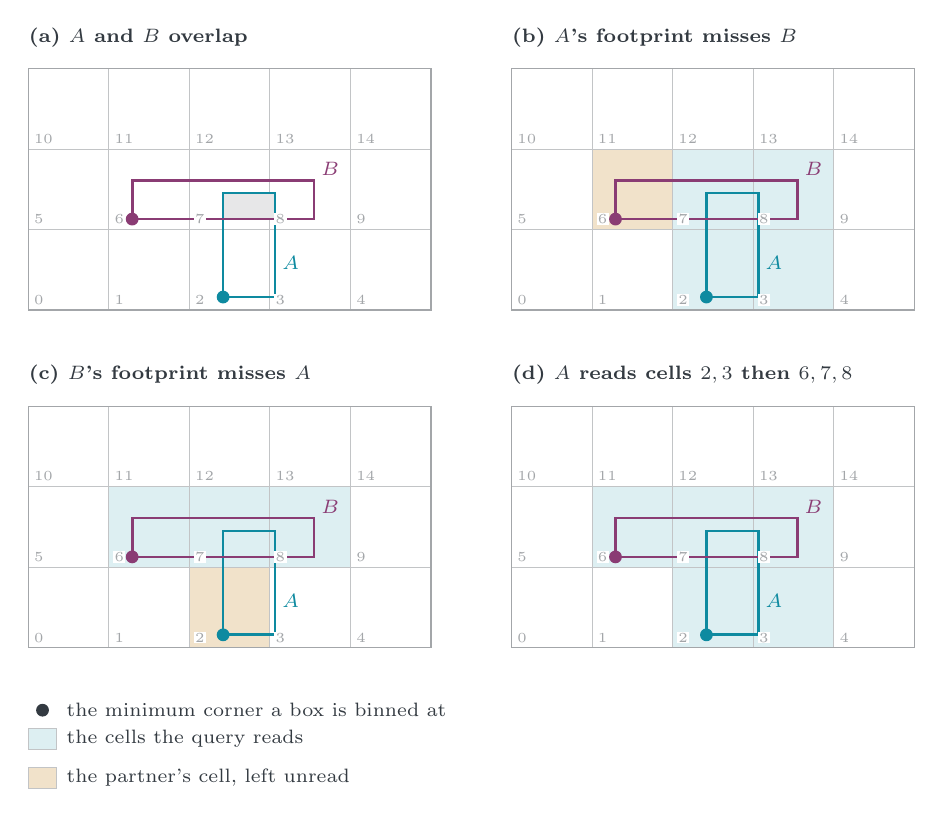
\begin{tikzpicture}[
  scale=1.65,
  font=\scriptsize,
  lbl/.style={font=\scriptsize, text=sccdInk, inner sep=1.5pt},
  tiny/.style={font=\tiny, text=sccdInk, inner sep=1pt},
  ttl/.style={font=\scriptsize\bfseries, text=sccdInk, inner sep=0pt},
  idle/.style={draw=sccdInk!22, line width=0.5pt},
  qbox/.style={draw=sccdTeal, line width=1.0pt},
  pbox/.style={draw=sccdPlum, line width=1.0pt},
  read/.style={fill=sccdTeal!14},
  unread/.style={fill=sccdAmber!22},
]

% A: minimum corner in column 2, row 0.  B: column 1, row 1.
\def\boxA{1.50/0.10/1.90/0.90}
\def\boxB{0.80/0.70/2.20/1.00}

\newcommand{\cellfill}[3]{%
  \fill[#3] ({#1*0.62},{#2*0.62}) rectangle ({(#1+1)*0.62},{(#2+1)*0.62});}

\newcommand{\scenegrid}{%
  \foreach \x in {0,0.62,1.24,1.86,2.48,3.10}
    \draw[draw=sccdInk!30, line width=0.3pt] (\x,0) -- (\x,1.86);
  \foreach \y in {0,0.62,1.24,1.86}
    \draw[draw=sccdInk!30, line width=0.3pt] (0,\y) -- (3.10,\y);
  \draw[draw=sccdInk!45, line width=0.4pt] (0,0) rectangle (3.10,1.86);}

\newcommand{\cellnumbers}{%
  \foreach \r in {0,1,2}
    \foreach \c in {0,1,2,3,4} {
      \pgfmathtruncatemacro{\id}{\r*5+\c}
      \node[tiny, text=sccdInk!45, anchor=south west, fill=white,
            inner sep=0.5pt] at ({\c*0.62+0.03},{\r*0.62+0.03}) {\id};}}

% The two boxes, with the minimum corner each is binned at.
\newcommand{\thetwoboxes}{%
  \foreach \xa/\ya/\xb/\yb in \boxA {
    \draw[qbox] (\xa,\ya) rectangle (\xb,\yb);
    \fill[sccdTeal] (\xa,\ya) circle (1.4pt);}
  \foreach \xa/\ya/\xb/\yb in \boxB {
    \draw[pbox] (\xa,\ya) rectangle (\xb,\yb);
    \fill[sccdPlum] (\xa,\ya) circle (1.4pt);}}

% ========================= (a) the two boxes =================================
\begin{scope}
  \node[ttl, anchor=south west] at (0,2.02) {(a) $A$ and $B$ overlap};

  \scenegrid
  % The overlap itself, so that the reader can see there is a pair to find.
  \fill[sccdInk!12] (1.50,0.70) rectangle (1.90,0.90);
  \thetwoboxes
  \cellnumbers
  \node[lbl, text=sccdTeal, anchor=north west] at (1.92,0.45) {$A$};
  \node[lbl, text=sccdPlum, anchor=south west] at (2.22,1.00) {$B$};
\end{scope}

% ===================== (b) A reads its own footprint =========================
% A is binned in cell 2 and its maximum corner in cell 8, so its footprint is
% columns 2-3 crossed with rows 0-1: cells 2, 3, 7, 8. B is binned in cell 6,
% one column to the left of that, and is never read.
\begin{scope}[shift={(3.72,0)}]
  \node[ttl, anchor=south west] at (0,2.02) {(b) $A$'s footprint misses $B$};

  \cellfill{2}{0}{read}  \cellfill{3}{0}{read}
  \cellfill{2}{1}{read}  \cellfill{3}{1}{read}
  \cellfill{1}{1}{unread}
  \scenegrid
  \thetwoboxes
  \cellnumbers
  \node[lbl, text=sccdTeal, anchor=north west] at (1.92,0.45) {$A$};
  \node[lbl, text=sccdPlum, anchor=south west] at (2.22,1.00) {$B$};
\end{scope}

% ===================== (c) B reads its own footprint =========================
% B is binned in cell 6 and its maximum corner in cell 8, so its footprint is
% columns 1-3 on row 1: cells 6, 7, 8. A is binned in cell 2, one row below,
% and is never read.
\begin{scope}[shift={(0,-2.60)}]
  \node[ttl, anchor=south west] at (0,2.02) {(c) $B$'s footprint misses $A$};

  \cellfill{1}{1}{read}  \cellfill{2}{1}{read}  \cellfill{3}{1}{read}
  \cellfill{2}{0}{unread}
  \scenegrid
  \thetwoboxes
  \cellnumbers
  \node[lbl, text=sccdTeal, anchor=north west] at (1.92,0.45) {$A$};
  \node[lbl, text=sccdPlum, anchor=south west] at (2.22,1.00) {$B$};
\end{scope}

% ===================== (d) the walk that does find it ========================
% A holds the smaller linear index, so it reports the pair. Its own row starts
% at its own cell; the row above starts where the row's prefix maximum says
% something reaches back, which is column 1 -- left of A's own column.
\begin{scope}[shift={(3.72,-2.60)}]
  \node[ttl, anchor=south west] at (0,2.02) {(d) $A$ reads cells $2,3$ then $6,7,8$};

  \cellfill{2}{0}{read}  \cellfill{3}{0}{read}
  \cellfill{1}{1}{read}  \cellfill{2}{1}{read}  \cellfill{3}{1}{read}
  \scenegrid
  \thetwoboxes
  \cellnumbers
  \node[lbl, text=sccdTeal, anchor=north west] at (1.92,0.45) {$A$};
  \node[lbl, text=sccdPlum, anchor=south west] at (2.22,1.00) {$B$};
\end{scope}

% ================================== key ======================================
\begin{scope}[shift={(0,-3.30)}]
  \fill[sccdInk] (0.11,0.22) circle (1.4pt);
  \node[lbl, anchor=west] at (0.26,0.22) {the minimum corner a box is binned at};
  \fill[read] (0.00,-0.08) rectangle ++(0.22,0.16);
  \draw[draw=sccdInk!30, line width=0.3pt] (0.00,-0.08) rectangle ++(0.22,0.16);
  \node[lbl, anchor=west] at (0.26,0.00) {the cells the query reads};
  \fill[unread] (0.00,-0.38) rectangle ++(0.22,0.16);
  \draw[draw=sccdInk!30, line width=0.3pt] (0.00,-0.38) rectangle ++(0.22,0.16);
  \node[lbl, anchor=west] at (0.26,-0.30) {the partner's cell, left unread};
\end{scope}
\end{tikzpicture}

  \caption{Why a query is not bounded by its own footprint, drawn to scale over
    a five-by-three grid of cells $0.62$ wide. \textbf{(a)} $A =
    [1.5,1.9]\times[0.1,0.9]$ is binned in cell $2$ and $B =
    [0.8,2.2]\times[0.7,1.0]$ in cell $6$; they overlap on both axes, shaded.
    $B$ begins a column to the left of $A$ and a row above it, so neither
    minimum-corner cell precedes the other componentwise.
    \textbf{(b)} $A$'s footprint is columns $2$--$3$ crossed with rows $0$--$1$,
    cells $2$, $3$, $7$ and $8$. It covers $B$'s row and not its column.
    \textbf{(c)} $B$'s footprint is columns $1$--$3$ on row $1$, cells $6$, $7$
    and $8$. It covers $A$'s column and not its row. Each misses the other by
    one coordinate, and no rule for deciding which box reports a pair recovers
    one that neither box reads.
    \textbf{(d)} Row-major linear index puts $A$ first, so $A$ reports. It reads
    its own row from its own cell, and the row above from column $1$, which the
    row's prefix maximum names because $B$ reaches back to $A$ from there ---
    left of $A$'s own column, which is the step (b) will not take.}
  \label{fig:incomparable}
\end{figure}

Row-major linear index $L(c_{0},c_{1}) = c_{1}n_{0} + c_{0}$ is \emph{total}, and
over it the walk is complete. For an overlapping pair $j$'s minimum does not pass
$i$'s maximum on either grid axis, so $L(\operatorname{cell}(j.\min)) \le
L(\operatorname{cell}(i.\max))$: the row term settles it when the rows differ and
the column does when they agree. Whichever box has the smaller $L$ therefore
holds the other in its range, and equal $L$ means one cell, where the index
decides --- the only index test in \cref{alg:cellmin}.

Read literally that range is whole rows, which is what the bounds are for. Each
cell carries the largest upper bound of the boxes in it and each row a prefix
maximum of those, so a binary search gives the first column holding anything that
reaches back to the querying box and the columns before it are skipped at once. That is a prefix maximum applied per row of cells, and it is what lets the
binning stand without a bound on how many cells a box may span; a grid that stores a box only at its lower-left
cell otherwise caps the box at $k$ cells and widens every query window by $k$ to
match. A second bound per cell does the same on the other axis.

\begin{algorithm}[htbp]
\caption{The edge-edge query, one pass (count or fill)}
\label{alg:cellmin}
\begin{algorithmic}[1]
\Function{EdgeToEdgeBroadPhase}{$A$}
  \State grid and cell size as in \cref{alg:cell}; bin each $A_{i}$ into
         $\operatorname{cell}(A_{i}.\min)$ alone
  \State $u_{c} \gets \max\{A_{j}.\max_{a_{1}} : j \in c\}$
    \Comment{$-\infty$ where $c$ is empty}
  \State $\mu_{c} \gets \max\{A_{j}.\max_{a_{0}} : j \in c',\; c' \le c \text{ in } \operatorname{row}(c)\}$
    \Comment{running maximum along each row}
  \ForAll{$i$ \textbf{in parallel}}
    \State $(c_{0}^{b},c_{1}^{b}) \gets \operatorname{cell}(A_{i}.\min)$;\quad
           $(c_{0}^{e},c_{1}^{e}) \gets \operatorname{cell}(A_{i}.\max)$
    \ForAll{$j$ listed in $(c_{0}^{b},c_{1}^{b})$ \textbf{with} $j > i$}
      \State \Call{Test}{$i$, $j$} \Comment{its own cell, where the index decides}
    \EndFor
    \For{$c_{1} \gets c_{1}^{b}$ \textbf{to} $c_{1}^{e}$}
      \If{$c_{1} = c_{1}^{b}$} $c_{0} \gets c_{0}^{b} + 1$
        \Comment{its own cell is read above}
      \Else{} $c_{0} \gets$ \Call{LowerBound}{$\mu$ on row $c_{1}$ up to $c_{0}^{e}$,
             $A_{i}.\min_{a_{0}}$}
      \EndIf
      \For{$c_{0}$ \textbf{to} $c_{0}^{e}$, cell $c \gets (c_{0},c_{1})$}
        \If{$u_{c} < A_{i}.\min_{a_{1}}$} \textbf{continue}
          \Comment{the cell is not read}
        \EndIf
        \ForAll{$j$ listed in $c$} \Call{Test}{$i$, $j$}
          \Comment{$c$ is ahead of $i$'s cell, so no index test}
        \EndFor
      \EndFor
    \EndFor
  \EndFor
\EndFunction
\Function{Test}{$i$, $j$}
  \If{$A_{i}$ and $A_{j}$ are disjoint in 3D, or share a vertex} \Return \EndIf
  \State count, or emit the pair
\EndFunction
\end{algorithmic}
\end{algorithm}

\begin{figure}[htbp]
  \centering
  % The edge-edge binning worked through on one scene: (a) the binning, then the
% walk of each box that emits a pair, in the order the cells put them.
%
% No prose inside the drawing. What the panels mean belongs in the caption,
% where it can be read at caption size and does not compete with the marks.
%
% Grids are drawn line by line rather than with TikZ's `grid`, which places its
% lines at multiples of the step measured from the origin and not from the
% corner of the rectangle given to it.
%
% The seven boxes and the grid are real: cells are 0.62 wide, six by four,
% numbered row-major from the bottom left, and every cell index, walk range and
% skipped column below follows from the coordinates in \scenebox.
% Drawn at 0.62 to the cell and scaled up to the text width. Coordinates scale,
% node text and line widths do not, so the panels grow and the labels keep their
% size -- which is why the panel offsets below are coordinates and not lengths.
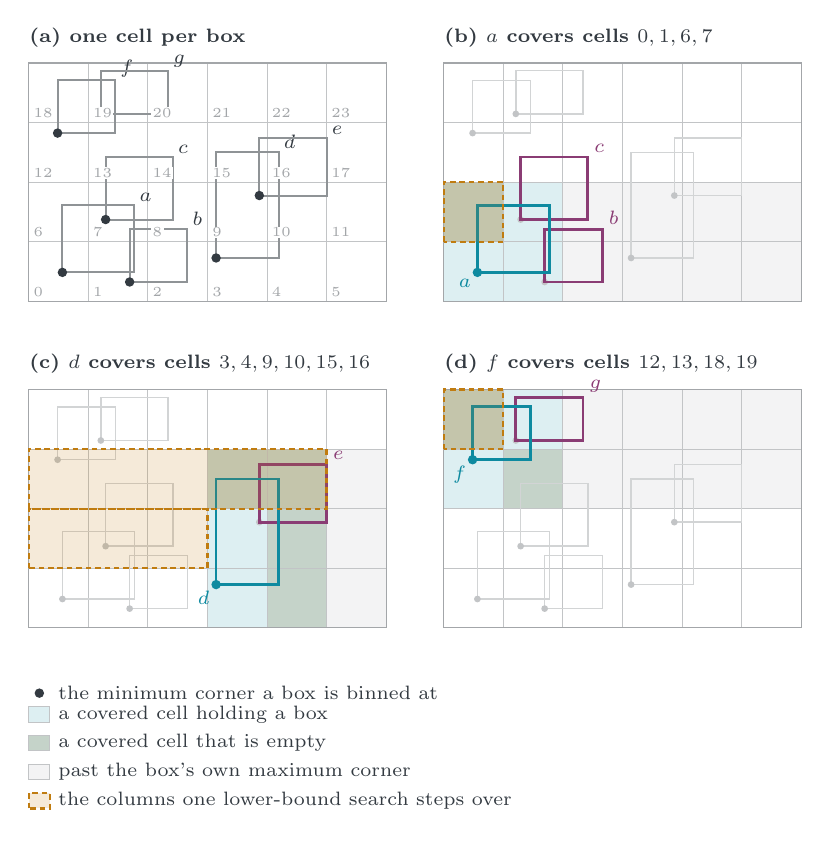
\begin{tikzpicture}[
  scale=1.22,
  font=\scriptsize,
  lbl/.style={font=\scriptsize, text=sccdInk, inner sep=1.5pt},
  tiny/.style={font=\tiny, text=sccdInk, inner sep=1pt},
  ttl/.style={font=\scriptsize\bfseries, text=sccdInk, inner sep=0pt},
  idle/.style={draw=sccdInk!22, line width=0.5pt},
  query/.style={draw=sccdTeal, line width=1.0pt},
  found/.style={draw=sccdPlum, line width=1.0pt},
  full/.style={fill=sccdTeal!14},
  empty/.style={fill=sccdMoss!30},
  beyond/.style={fill=sccdInk!6},
  % The span one binary search over the row's prefix maximum steps over. The
  % tint is translucent so the cell fills beneath it still read: a searched cell
  % can be covered, empty, or neither.
  search/.style={draw=sccdAmber, line width=0.8pt,
                 dash pattern=on 2pt off 1.4pt,
                 fill=sccdAmber, fill opacity=0.16},
]

% The columns a row's lower-bound search steps over, as c0..c1 on row r.
\newcommand{\searchspan}[3]{%
  \draw[search] ({#1*0.62},{#3*0.62}) rectangle ({(#2+1)*0.62},{(#3+1)*0.62});}

% One cell, addressed by column and row.
\newcommand{\cellfill}[3]{%
  \fill[#3] ({#1*0.62},{#2*0.62}) rectangle ({(#1+1)*0.62},{(#2+1)*0.62});}

% label / x0 / y0 / x1 / y1 -- the minimum corner is (x0,y0).
\def\scenebox{%
  a/0.35/0.30/1.10/1.00, b/1.05/0.20/1.65/0.75, c/0.80/0.85/1.50/1.50,
  d/1.95/0.45/2.60/1.55, e/2.40/1.10/3.10/1.70, f/0.30/1.75/0.90/2.30,
  g/0.75/1.95/1.45/2.40}

% The grid, drawn line by line. #1 is unused; kept as a command for brevity.
\newcommand{\scenegrid}{%
  \foreach \x in {0,0.62,1.24,1.86,2.48,3.10,3.72}
    \draw[draw=sccdInk!30, line width=0.3pt] (\x,0) -- (\x,2.48);
  \foreach \y in {0,0.62,1.24,1.86,2.48}
    \draw[draw=sccdInk!30, line width=0.3pt] (0,\y) -- (3.72,\y);
  \draw[draw=sccdInk!45, line width=0.4pt] (0,0) rectangle (3.72,2.48);}

% Every box in the faint style, then the minimum corner each is binned at.
\newcommand{\sceneidle}{%
  \foreach \n/\xa/\ya/\xb/\yb in \scenebox {
    \draw[idle] (\xa,\ya) rectangle (\xb,\yb);
    \fill[sccdInk!30] (\xa,\ya) circle (1.0pt);}}

% ============================ (a) the binning ================================
\begin{scope}
  \node[ttl, anchor=south west] at (0,2.64) {(a) one cell per box};

  \scenegrid
  \foreach \n/\xa/\ya/\xb/\yb in \scenebox {
    \draw[draw=sccdInk!55, line width=0.7pt] (\xa,\ya) rectangle (\xb,\yb);
    \fill[sccdInk] (\xa,\ya) circle (1.4pt);
    \node[lbl, anchor=south west, inner sep=1pt] at ({\xb+0.02},\yb) {$\n$};}

  % Cell numbers last, so no box can hide one, and in the corner the box labels
  % do not use.
  \foreach \r in {0,1,2,3}
    \foreach \c in {0,1,2,3,4,5} {
      \pgfmathtruncatemacro{\id}{\r*6+\c}
      \node[tiny, text=sccdInk!45, anchor=south west, fill=white,
            inner sep=0.5pt] at ({\c*0.62+0.03},{\r*0.62+0.03}) {\id};}
\end{scope}

% ============================= (b) box a walks ===============================
% a is binned in cell 0 and its maximum corner in cell 7, so it covers cells 0,
% 1, 6 and 7 -- rows 0-1 crossed with columns 0-1. On row 1 the running maximum
% starts the scan at column 1: cell 6 is empty, so nothing there reaches back.
\begin{scope}[shift={(4.32,0)}]
  \node[ttl, anchor=south west] at (0,2.64) {(b) $a$ covers cells $0,1,6,7$};

  \cellfill{0}{0}{full}  \cellfill{1}{0}{full}  \cellfill{1}{1}{full}
  \cellfill{0}{1}{empty}
  \fill[beyond] (1.24,0) rectangle (3.72,1.24);
  \scenegrid
  \sceneidle

  \draw[found] (1.05,0.20) rectangle (1.65,0.75);
  \draw[found] (0.80,0.85) rectangle (1.50,1.50);
  \draw[query] (0.35,0.30) rectangle (1.10,1.00);
  \fill[sccdTeal] (0.35,0.30) circle (1.4pt);
  % Row 1: the search starts the row at column 1, stepping over cell 6.
  \searchspan{0}{0}{1}

  \node[lbl, text=sccdPlum, anchor=south west] at (1.67,0.75) {$b$};
  \node[lbl, text=sccdPlum, anchor=south west] at (1.52,1.50) {$c$};
  \node[lbl, text=sccdTeal, anchor=north east] at (0.33,0.28) {$a$};
\end{scope}

% ============================= (c) box d walks ===============================
% d is binned in cell 3 and its maximum corner in cell 16, so it covers cells 3,
% 4, 9, 10, 15 and 16 -- rows 0-2 crossed with columns 3-4. Row 2 holds only f,
% whose maximum on the first axis is 0.90 and so never reaches d: the running
% maximum returns a column past 4 and the whole row is skipped without being
% read.
\begin{scope}[shift={(0,-3.40)}]
  \node[ttl, anchor=south west] at (0,2.64) {(c) $d$ covers cells $3,4,9,10,15,16$};

  % Only 3 and 9 hold anything: d itself and e. Cells 4 and 10 are read and
  % yield nothing, and 15 and 16 are stepped over by the running maximum.
  \cellfill{3}{0}{full}  \cellfill{3}{1}{full}
  \cellfill{4}{0}{empty} \cellfill{4}{1}{empty}
  \cellfill{3}{2}{empty} \cellfill{4}{2}{empty}
  \fill[beyond] (3.10,0) rectangle (3.72,1.86);
  \scenegrid
  \sceneidle

  \draw[found] (2.40,1.10) rectangle (3.10,1.70);
  \draw[query] (1.95,0.45) rectangle (2.60,1.55);
  \fill[sccdTeal] (1.95,0.45) circle (1.4pt);
  % Row 1: the search steps over columns 0-2, left of $d$'s own columns, where a
  % partner binned lower could still reach back. Row 2: it returns a column past
  % 4 and steps over the whole row.
  \searchspan{0}{2}{1}
  \searchspan{0}{4}{2}

  \node[lbl, text=sccdPlum, anchor=south west] at (3.12,1.70) {$e$};
  \node[lbl, text=sccdTeal, anchor=north east] at (1.93,0.43) {$d$};
\end{scope}

% ============================= (d) box f walks ===============================
% f is binned in cell 12 and its maximum corner in cell 19, so it covers cells
% 12, 13, 18 and 19 -- rows 2-3 crossed with columns 0-1. On row 3 the running
% maximum starts at column 1, cell 18 being empty.
\begin{scope}[shift={(4.32,-3.40)}]
  \node[ttl, anchor=south west] at (0,2.64) {(d) $f$ covers cells $12,13,18,19$};

  \cellfill{0}{2}{full}  \cellfill{1}{3}{full}
  \cellfill{1}{2}{empty} \cellfill{0}{3}{empty}
  \fill[beyond] (1.24,1.24) rectangle (3.72,2.48);
  \scenegrid
  \sceneidle

  \draw[found] (0.75,1.95) rectangle (1.45,2.40);
  \draw[query] (0.30,1.75) rectangle (0.90,2.30);
  \fill[sccdTeal] (0.30,1.75) circle (1.4pt);
  % Row 3: the search starts the row at column 1, stepping over cell 18.
  \searchspan{0}{0}{3}

  \node[lbl, text=sccdPlum, anchor=south west] at (1.47,2.40) {$g$};
  \node[lbl, text=sccdTeal, anchor=north east] at (0.28,1.73) {$f$};
\end{scope}

% ================================== key ======================================
\begin{scope}[shift={(0,-4.30)}]
  \fill[sccdInk] (0.11,0.22) circle (1.4pt);
  \node[lbl, anchor=west] at (0.26,0.22) {the minimum corner a box is binned at};
  \fill[full] (0.00,-0.08) rectangle ++(0.22,0.16);
  \draw[draw=sccdInk!30, line width=0.3pt] (0.00,-0.08) rectangle ++(0.22,0.16);
  \node[lbl, anchor=west] at (0.26,0.00) {a covered cell holding a box};
  \fill[empty] (0.00,-0.38) rectangle ++(0.22,0.16);
  \draw[draw=sccdInk!30, line width=0.3pt] (0.00,-0.38) rectangle ++(0.22,0.16);
  \node[lbl, anchor=west] at (0.26,-0.30) {a covered cell that is empty};
  \fill[beyond] (0.00,-0.68) rectangle ++(0.22,0.16);
  \draw[draw=sccdInk!30, line width=0.3pt] (0.00,-0.68) rectangle ++(0.22,0.16);
  \node[lbl, anchor=west] at (0.26,-0.60) {past the box's own maximum corner};
  \draw[search] (0.00,-0.98) rectangle ++(0.22,0.16);
  \node[lbl, anchor=west] at (0.26,-0.90)
    {the columns one lower-bound search steps over};
\end{scope}
\end{tikzpicture}

  \caption{The edge-edge binning run through on one scene, drawn to scale: every
    cell index, walk range and skipped span below follows from the coordinates
    shown. \textbf{(a)} Seven swept boxes over a six-by-four grid, each binned
    into the one cell holding its minimum corner --- $a$ into cell $0$, $b$ into
    $1$, $d$ into $3$, $c$ into $7$, $e$ into $9$, $f$ into $12$ and $g$ into
    $19$, the cells numbered row-major from the bottom left. Four pairs of these
    boxes overlap, and each is emitted by whichever of the two sits in the lower
    cell, so only three of the seven boxes emit anything.
    \textbf{(b)} $a$ covers cells $0$, $1$, $6$ and $7$, the last holding its
    maximum corner, and finds $b$ and $c$ in $1$ and $7$. Cell $6$ is empty, so
    the running maximum starts that row at the next column and the cell is never
    read. A run of empty cells costs one binary search and not a test per cell.
    \textbf{(c)} $d$ covers cells $3$, $4$, $9$, $10$, $15$ and $16$, of which
    $3$ holds $d$ itself and $9$ holds $e$, the pair it emits. Cells $4$ and
    $10$ are read and yield nothing. The third row is skipped whole, the empty
    cells $15$ and $16$ included although $d$ covers them: the
    only box binned in that row is $f$, which ends well to the left of where $d$
    begins, so one search puts the row past $d$'s own maximum column and it is
    never entered. Past its own row the walk also reaches left of its own
    columns, because a box binned in a lower column can still be wide enough to
    reach back into $d$ and $d$ holds the lower cell, so that pair would be its
    to report; those cells are skipped by the same search and are left unmarked
    here, being too far from $d$ for the drawing to say anything about them.
    \textbf{(d)} $f$ covers cells $12$, $13$, $18$ and $19$, and finds $g$ in
    $19$; of the two empty cells $13$ is read and $18$ the search steps over.
    $b$, $c$, $e$ and $g$ walk too, and emit
    nothing: each of their partners sits in a lower cell and has already
    reported the pair.}
  \label{fig:cellmin}
\end{figure}

Cost follows the same two terms as \cref{alg:cell}, with the binning reduced to
one incidence per box and the query to whatever the bounds leave. Ordering each
cell's entries on the axis the
grid does not use would make the scan inside a cell monotone as well --- a grid
and sweep-and-prune hybrid of the kind \citet{serpa2020broadmark} evaluates. It
culls where cells are densely occupied and pays an ordering pass everywhere, and
on our scenes the two roughly cancel, so the cells are left unordered.

\section{Narrow phase}
\label{sec:np}

Each candidate pair that survives \cref{sec:bp} is decided here, by branch and
bound over boxes in the parameter domain. Two properties from \cref{sec:prelim}
make the search possible at all. \Cref{eq:hull} says that a box can be judged
from its eight corners, and \cref{eq:err} says by how much that judgement can be
wrong. \Cref{alg:np} is the skeleton every kernel in this paper instantiates.
Three things vary between them: the acceptance test, the split rule, and how the
work list is organised. The third is the subject of \cref{sec:parallel}.

\begin{algorithm}[htbp]
\caption{Branch and bound for one query. $\toi$ is the running minimum, shared
across queries when the caller asks only for the earliest impact.}
\label{alg:np}
\begin{algorithmic}[1]
\Function{NarrowPhase}{query, $\toi$}
  \State $\epsilon \gets$ error bound of \cref{eq:err};\quad
         $\tau_{0..2} \gets$ tolerances of \cref{eq:tol}
  \State push $\dom_{0} = [0,\min(\toi,1)]\times[0,1]^{2}$
  \While{a box $\dom$ remains}
    \If{$\dom.t_{\ell} \ge \toi$} \textbf{continue}
      \Comment{a root here cannot improve the answer}
    \EndIf
    \State $[\,\underline{F}_{d},\overline{F}_{d}\,] \gets$ hull of the eight
           corner values, per component \Comment{\cref{eq:hull}}
    \If{$\underline{F}_{d} > \epsilon_{d}$ or $\overline{F}_{d} < -\epsilon_{d}$
        for any $d$}
      \State \textbf{continue} \Comment{\textbf{reject}: the only unsound step,
             so it is padded by $\epsilon$}
    \EndIf
    \If{\Call{Accept}{$\dom$} \textbf{or} $\dom.\text{depth} \ge D$
        \textbf{or} $\dom$ cannot be split}
      \State $\toi \gets \min(\toi,\ \dom.t_{\ell})$;\quad \textbf{continue}
        \Comment{exhaustion \emph{accepts}, never drops}
    \EndIf
    \State push the children of \Call{Split}{$\dom$}
  \EndWhile
  \State \Return $\toi$
\EndFunction
\end{algorithmic}
\end{algorithm}

On acceptance \cref{alg:np} reports the \emph{lower} bound in $t$ of the
accepted box, never its midpoint and never its upper bound. Every exit that is
not a rejection accepts. Those two facts are the whole of the safety argument,
and \cref{sec:guarantee} makes them precise.

\subsection{Two acceptance tests}
\label{sec:np:modes}

Two instantiations of \op{Accept} and \op{Split} appear in what follows. Both
are conservative. They differ in how tight an answer they return, and in how
long they take to return it.

The first, \textsc{Tight}, is TightInclusion's test transcribed:
\begin{equation} \label{eq:accept-tight} \textsc{Accept}(\dom) \;=\;
\underbrace{\bigl(\forall d:\ [\underline{F}_{d},\overline{F}_{d}] \subseteq
[-\epsilon_{d},\epsilon_{d}]\bigr)}_{\text{function box inside the error box}}
\ \vee\ \underbrace{\bigl(\forall k:\ \dom.w_{k} \le
\tau_{k}\bigr)}_{\text{\emph{domain} width within \emph{domain} tolerance}} ,
\end{equation} and its split halves the axis furthest past its own tolerance,
$\arg\max_{k} \dom.w_{k}/\tau_{k}$. The search starts from $[0,1]^{3}$, so
every midpoint is a dyadic rational, and it is exact in binary floating point
while the depth stays below the width of the significand. The implementation
does not assume that. It checks that the midpoint separates the endpoints, and
accepts the box when it does not.

The second, \textsc{Relaxed}, accepts on a \emph{codomain} width measured
against a \emph{domain} tolerance, $\forall d:
\overline{F}_{d}-\underline{F}_{d} \le \tau_{d}$. It adds the same error-box
condition and two degenerate cases. Comparing quantities that carry different
units makes the test loose, so it accepts earlier and reports a time of impact
further before the true one. \Cref{sec:results:relaxed} quantifies that trade,
which does not run one way.

Both tests also require $\dom.t_{\ell} > 0$. That refuses a contact reported at
exactly $t=0$, which would stall a solver using $\toi$ as a step length.
Measured against the exact roots the condition costs nothing: with it in place,
no collision is missed and no time of impact is late.

\subsection{The adaptive splitter, and what measuring it showed}
\label{sec:np:split}

\textsc{Relaxed} and the quad kernel split an axis several ways at once. The chosen axis is cut at $N=2$ interior points, giving three
children. Each point comes from a one-dimensional Gauss--Newton step against the
linearisation of $\Fdiff$ along that axis, clamped to within $0.45h$ of its
nominal position, where $h$ is the uniform spacing. The splitter is about
$1.6\times$ faster than a uniform grid, which needs five sub-intervals where
this uses three. Measuring \emph{why} produced a more useful result than the
speedup did.

First, the splitter barely adapts. The nominal point cancels exactly from the
Gauss--Newton step, so all $N$ splitters solve for the same least-squares point.
They differ only in which clamp window each one lands in, and $95.9\%$ of them
are pinned at their clamp. The clamp, and not the Newton step, is what makes
each child a bounded fraction of its parent. An unclamped version fails to
terminate.

Second, placement cannot affect correctness: the children tile the parent and
every child is still tested, so the splitter is purely a performance knob.

Third, and most informative, a principled alternative \emph{lost}. A
chord-based splitter aimed at the largest root-free region ran $2.7\times$
slower and isolated \emph{less} dead volume, $56.7\%$ against $61.1\%$. The
cause is a mismatch between what is dead and what is rejectable. On a typical
parent, $68.4\%$ of the volume is root-free \emph{pointwise}, taken as a union
over the three components of $\Fdiff$. Rejecting a child, however, requires a
\emph{single} component to exclude the origin over the whole child, and only
about $58\%$ of the axis is rejectable that way. A multi-way split does better
because different children may die by different components. A single
well-placed cut has no such advantage.

\subsection{Order independence}
\label{sec:np:order}

TightInclusion pops boxes from a priority queue ordered by ascending $t$ lower
bound, and returns the first box it accepts. Its answer is therefore the
accepted box of globally smallest $t$. \Cref{alg:np} keeps no such order. The
proposition below says that it needs none, and it is the result that licenses
everything in \cref{sec:parallel}.

\begin{proposition}[Order independence]
\label{prop:order}
Let $\mathcal{A}$ be the set of boxes that \op{Accept} accepts, over the tree
generated by a fixed \op{Split}. Suppose a search explores that tree in any
order, maintains $\toi = \min\{\dom.t_{\ell} : \dom \in \mathcal{A}
\text{ reached}\}$, and skips any box with $\dom.t_{\ell} \ge \toi$. Then on
termination $\toi = \min\{\dom.t_{\ell} : \dom \in \mathcal{A}\}$, independent of
the exploration order.
\end{proposition}

\begin{proof}
Let $m$ be the right-hand side and $\dom^{\ast}$ a box attaining it. Since $\toi$
only ever takes values $\dom.t_{\ell}$ for reached $\dom \in \mathcal{A}$, we
have $\toi \ge m$ throughout. For the converse, suppose $\dom^{\ast}$ is skipped.
It is skipped only because $\dom^{\ast}.t_{\ell} \ge \toi$ at that moment, and
$\toi \ge m = \dom^{\ast}.t_{\ell}$, so $\toi = m$ already. Otherwise
$\dom^{\ast}$ is reached and $\toi \le \dom^{\ast}.t_{\ell} = m$. The same
argument applies to every ancestor of $\dom^{\ast}$: an ancestor is pruned only
when $\toi$ has already reached a value at or below its $t$ lower bound, which is
at or below $m$. Hence $\toi = m$ in all cases.
\end{proof}

\begin{remark}[Agreement with the reference]
\label{rem:ti}
TightInclusion's answer is the same minimum, so the two agree exactly. Its queue
is ordered by ascending $t$ lower bound, so the first accepted box it pops has the
smallest $t$ lower bound among accepted boxes it \emph{reaches}; and a box it
does not reach was pruned by the same $t$ bound, which by the argument above is
already at or below that minimum. Hence its answer is
$\min\{\dom.t_{\ell} : \dom \in \mathcal{A}\}$, the same quantity
\cref{prop:order} gives.
\end{remark}

The hypotheses of \cref{prop:order} are not a formality. It fixes \op{Accept}
and \op{Split}, and so fixes $\mathcal{A}$. Two searches agree only when they
generate the same $\mathcal{A}$, and that requires the same acceptance
\emph{rule} together with the same computed values feeding it, down to the last
bit.

Our host kernel and TightInclusion meet that condition. The corner evaluation is
written in the reference's expression order precisely so that they do
(\cref{sec:prelim:err}). \Cref{sec:results:ref} confirms the consequence to
every printed digit on all twelve scene-phases, which is the sharpest check of
the proposition available to us.

Our \emph{device} kernel does not meet it. It evaluates the same formulas
through vector fused multiply-adds, and it rounds $\delta^{3}$ upward with a plain cube. A box decided in the last few units in the last place
can therefore fall differently, and its $\mathcal{A}$ is a slightly different
set. \Cref{prop:order} thus explains why the host reproduces the reference, and
says nothing about how closely the device will. \Cref{sec:results:ref} measures
that separately, and the answer is close without being identical.

What the proposition buys is freedom. The traversal may be depth-first,
breadth-first, or interleaved across queries; boxes from unrelated queries may
share a vector register or a thread block; work may migrate between processors
mid-search. None of that can change the answer. The two implementations in
\cref{sec:parallel} spend that freedom in different currencies.

\subsection{Quads}
\label{sec:np:quad}

Quad meshes are handled directly, without triangulation. They have their own
inclusion function (\cref{eq:fvq}), their own tolerance and error reductions,
their own host root finder and their own device kernel.

This path is \emph{not evaluated} in this paper. Every scene in
\cref{sec:results} is a triangle mesh, so no measurement reported here bears on
a quad, and the error constant of \cref{sec:prelim:err} for the bilinear form is
uncertified. What follows is a design, verified for correctness against a
densely sampled reference root and against the alternative factoring below. It
is not a measured result.

We considered extending the triangle kernel and rejected it. That kernel is
built end to end around a four-point query packed into one vector register, on a
barycentric domain whose validity test rejects $u+v \ge 1$. A vertex-quad query
has five points on an independent domain, so the load, the tolerances, the error
bound, the corner evaluation, the domain test and the split would all have had
to change at once.

Two details of the implementation matter. The first is the factoring. The
evaluation is written $\Fdiff = q(t) - \sum_{k} w_{k}(u,v)\,g_{k}(t)$, and not
as a blend in $(u,v)$ first, because the weights do not depend on $t$. A split
along $u$ or $v$ then holds the $t$-dependent frame fixed across every corner it
evaluates, so the frame is computed once for the whole split.

The second is the node order, which in \cref{eq:fvq} is lexicographic and not
cyclic. Winding the nodes around the quad swaps the last two. The solver then
searches a bilinear saddle stretched across the diagonal, and reports a
perfectly valid time of impact for a surface the caller did not mean. That
failure is silent, which is why we state the convention here and not in a
manual.

One further measurement from the quad path generalises. Hoisting the evaluation
of the split planes out of the loop over children is the textbook optimisation.
It is $1.3\times$ faster per isolated query and $1.35\times$ slower end to end.
The cause is that $\toi$ sharpens \emph{during} the loop. A child whose $t$
lower bound has since passed the running minimum is discarded unlooked-at, and
hoisting evaluates it anyway. When the bound is shared, a loop-invariant
computation is not invariant in the only sense that matters.

\section{Parallel implementation}
\label{sec:parallel}

\Cref{prop:order} says the search tree may be explored in any order, which
leaves the traversal free to be organised around the processor rather than
around the query. Both implementations use that freedom, and they use it in
opposite directions. The host kernel fills the lanes of one vector register with
boxes drawn from different queries, so a lane never idles while its neighbours
work (\cref{sec:parallel:host}). The device kernel does the reverse: it moves
boxes \emph{out} of the block that produced them, into a queue that the next
launch spreads over the whole device (\cref{sec:parallel:device}). The broad
phase needs no such treatment, since its parallelism is already the outermost
loop of \cref{alg:cell,alg:cellmin} and its count-then-fill output carries no
contention.

What both designs answer is a single property of the problem: the cost of a CCD
query is heavy-tailed. Most candidate pairs are settled by the first box the
search looks at, while a few require tens of thousands or more
(\cref{tab:difficulty}, at the end of this section). A design that pins one
query to one execution resource --- a lane, a thread, a block --- is therefore
load-imbalanced by construction, and not by a factor of two. The remainder of
this section presents the two kernels and the parameters they were measured at;
\cref{sec:parallel:why} returns to the measurement and to what the two
distributions say about where the work goes.

\subsection{Host: lanes packed across queries}
\label{sec:parallel:host}

The unit of work on the host is the \emph{box}, not the query. A vector of $V$
lanes ($V=8$ on AVX-512 and AVX2, $4$ on NEON) holds $V$ boxes that may belong
to $V$ different queries, and the kernel advances all of them through one
iteration of \cref{alg:np} together. Queries are processed in blocks of $V$
consecutive candidates, one block per task of the parallel loop; a block's
geometry, per-axis tolerances and certified error bound are computed once on
entry, and each query contributes the root box $[0,\toi]\times[0,1]^{2}$ to a
work list private to the block. A lane that decides its box takes the next box
off that list, whichever query it belongs to, and the lane's geometry is
reloaded only when the query actually changes. \Cref{prop:order} is what makes
this legal: the answer does not depend on the order in which boxes are visited,
so interleaving unrelated queries in one register cannot change it.

One iteration proceeds in three phases, and the division is what allows a single
flat vector sweep to serve lanes that are doing different things.

\emph{Classify} decides the fate of every lane from quantities it already
carries. Each box stores the value of $\Fdiff$ at its eight corners, so the
componentwise hull of \cref{eq:hull} is a min and a max over stored values, taken
across all lanes at once, and no function evaluation occurs in this phase at all.
A lane whose hull excludes the origin by more than the certified bound is
rejected and goes idle; a lane that the acceptance test of
\cref{eq:accept-tight} accepts, or that has reached the depth cap, or whose box
can no longer be bisected in floating point, lowers its query's running minimum
to the box's $t$ lower bound and goes idle. Every remaining lane chooses its
split axis, the one furthest past its own tolerance, and the midpoint of that
axis.

\emph{Evaluate} is the only phase that computes $\Fdiff$. A bisection cuts the
parent at a mid-face, so the two children share that face and each inherits its
outer face from the parent: the four corner values of the mid-face are all that
the split needs. Those four parameter triples are laid out for every splitting
lane and evaluated in one vector sweep, even though the lanes are splitting
different axes --- the axis enters only through which parent coordinates are
written into the sweep's input, so the arithmetic is identical across lanes.
Lanes that are not splitting ride along and their results are discarded, which
is cheaper than branching inside the loop.

\emph{Assemble} forms the two children from the parent's corners and the newly
evaluated mid-face. The upper child goes to the work list; the lower child stays
in the lane, overwriting its parent in place. Keeping the lower child is what
makes each lane depth-first in $t$: the child that may contain an earlier impact
is examined first, so the running minimum falls sooner and prunes harder, the
work list carries half the traffic, and the lane needs no refill and no geometry
reload. Either child is dropped before it is written if the running minimum has
already passed its $t$ lower bound, or --- for a vertex-face query, whose domain
is the triangle $u+v\le1$ rather than the unit square --- if the child lies
outside that domain. When the block is exhausted, its per-query minima are either
written out per pair or folded into the shared minimum by compare-and-swap,
according to what the caller asked for.

\begin{algorithm}[!tb]
\caption{Host narrow phase. Lanes hold boxes from different queries, which
\cref{prop:order} permits. $V$ is the vector width and $D$ the depth cap.}
\label{alg:host}
\footnotesize
\begin{algorithmic}[1]
\Function{HostNarrowPhase}{candidates $\Cand$}
  \ForAll{blocks $Q$ of $V$ consecutive queries \textbf{in parallel}}
    \State load geometry, $\tau$ and $\epsilon$ per query;\;
           $\toi_{q} \gets$ shared minimum, or $1$ when the caller wants one
           answer per pair
    \State $S \gets$ work list holding each query's root box with its $8$
           corner values
    \State all $V$ lanes idle
    \While{true}
      \ForAll{idle lanes $l$}
        \Comment{refill}
        \State pop $\dom$ from $S$, discarding any with
               $\dom.t_{\ell} \ge \toi_{\dom.q}$
        \State bind $\dom$ to lane $l$, reloading lane geometry only if
               $\dom.q$ changed
      \EndFor
      \State \textbf{if} no lane holds a box \textbf{then break}
      \State $[\underline{F},\overline{F}] \gets$ hull of the $8$ stored
             corners, per component, all lanes at once
      \ForAll{lanes $l$ holding a box}
        \Comment{phase 1: classify, evaluating nothing}
        \If{$\dom_{l}$ is rejected by the test of \cref{eq:err}}
          \State lane $l \gets$ idle
        \ElsIf{\Call{Accept}{$\dom_{l}$} \textbf{or} $\mathrm{depth}_{l} \ge D$
               \textbf{or} $\dom_{l}$ cannot be bisected}
          \State $\toi_{q_{l}} \gets \min(\toi_{q_{l}},\ \dom_{l}.t_{\ell})$;\;
                 lane $l \gets$ idle
        \Else
          \State $a_{l} \gets \arg\max_{k} \dom_{l}.w_{k}/\tau_{k}$;\;
                 $m_{l} \gets$ midpoint of axis $a_{l}$
        \EndIf
      \EndFor
      \State lay out the $4$ mid-face corner parameters of every splitting lane
      \State evaluate $\Fdiff$ there in \emph{one} vector sweep across all lanes
        \Comment{phase 2}
      \ForAll{splitting lanes $l$}
        \Comment{phase 3: assemble}
        \State push the upper child onto $S$: the parent's outer face, the new
               mid face
        \State keep the lower child in lane $l$, overwritten in place
          \Comment{depth-first in $t$}
        \State discard either child whose $t$ lower bound has passed
               $\toi_{q_{l}}$, or which leaves the query's domain
      \EndFor
    \EndWhile
    \State write $\toi_{q}$ out, or lower the shared minimum by
           compare-and-swap
  \EndFor
\EndFunction
\end{algorithmic}
\end{algorithm}

\subsection{Device: a small stack, and a queue that redistributes}
\label{sec:parallel:device}

The device kernel runs one thread per query and one launch per round of work. A
launch is given a set of boxes, searches them to completion without ever waiting
for another launch, and writes the boxes it could not keep into a queue in global
memory; the host then relaunches the same kernel on that queue. Within a launch
the unit of work is again the box: a thread that finishes its own query's subtree
takes a box belonging to any query from a stack its block shares, and reloads
geometry only if the query changed. \Cref{fig:gpu-workflow} shows the two levels
of storage and \cref{alg:device} gives both the kernel and the host loop around
it.

The per-block stack lives in shared memory and holds $64$ entries, which is
small on purpose. The stack is where a query's subtree accumulates, so its
capacity decides how long a block keeps a heavy query to itself: with room for a
thousand boxes a single block grinds through a query of tens of thousands
(\cref{tab:difficulty}) while its neighbours finish and idle, and no other block
can help, because nothing the block holds is visible outside it. Spilling after $64$ entries pushes that
subtree into the global queue instead, where the next launch distributes it over
every block on the device. The effect is large and it is a scheduling effect, not
a pruning one: the false positives and the reported times of impact are identical
at every capacity (\cref{sec:parallel:tuning}).

The global queue is double buffered. A launch reads one half and writes the
other, never both, so a producer and its consumer are always in different
launches and no thread ever waits on another thread's progress. This is the
reason the queue is organised in rounds at all rather than as a single shared
work pool: a pool whose writers spin on a compare-and-swap until a reader frees a
slot deadlocks as soon as the queue is driven hard, which is precisely the
condition that redistributing work creates. The host loop therefore alternates:
it reads the write cursor after each launch and relaunches on what that launch
produced, swapping the roles of the two halves, until a round produces nothing.

A box that does not fit in the write buffer is counted and discarded. Discarding
is sound rather than merely convenient: every exit from the search other than a
rejection accepts the box at its $t$ lower bound, so a box never examined can
only leave the reported time of impact earlier than the truth, never later
(\cref{sec:np}) --- the failure direction that matters is closed by
construction, and what an undersized queue costs is accuracy. The host reads the
deficit, enlarges the queue by exactly that many entries and reruns the batch
from its seeds, keeping the times of impact already found so that the rerun
prunes harder. Growth is by the deficit rather than geometric because every call
clears the queue it is given, so an oversized queue is paid for on every
subsequent call and not once; the retry is bounded at $32$ rounds, after which
the kernel reports the shortfall and stops, since giving up is conservative and
spinning is not finite.

A work list that is meant never to overflow can be sized from the search rather
than from a measurement, which is what the vertex-quad kernel does with its
per-thread stack: a pop pushes at most $k$ children, so a depth-$D$ search needs
at most $1+kD$ entries for one query, and the headroom is nearly free --- a
$257$-entry frame is $14.7\,\mathrm{KB}$ of which only the first few entries are
ever touched, and register count and spill are unchanged between capacities $4$
and $513$. The shared stack above is the opposite case and is sized against that
rule on purpose: it is not meant to hold a query's frontier, only to pass it on.

The device broad phase is a more conventional port of \cref{alg:cell,alg:cellmin}:
count, prefix sum and scatter, with a radix sort and a device scan from
CUB~\citep{cub} in place of their host equivalents, one box per thread, and a
scalar inner loop where the host uses its $32$-lane mask. Its shape suits a GPU
because no part of it walks a window sequentially.

\begin{figure}[htbp]
  \centering
  \resizebox{0.86\linewidth}{!}{% The device narrow phase's work flow: a small per-block shared stack that spills
% early into a double-buffered global queue, which the next launch redistributes.
%
% Every node carries an explicit inner sep so its text keeps a margin from its
% frame, group labels are placed outside the group they name, and arrows are
% shortened at both ends so no head or tail lands on a border.
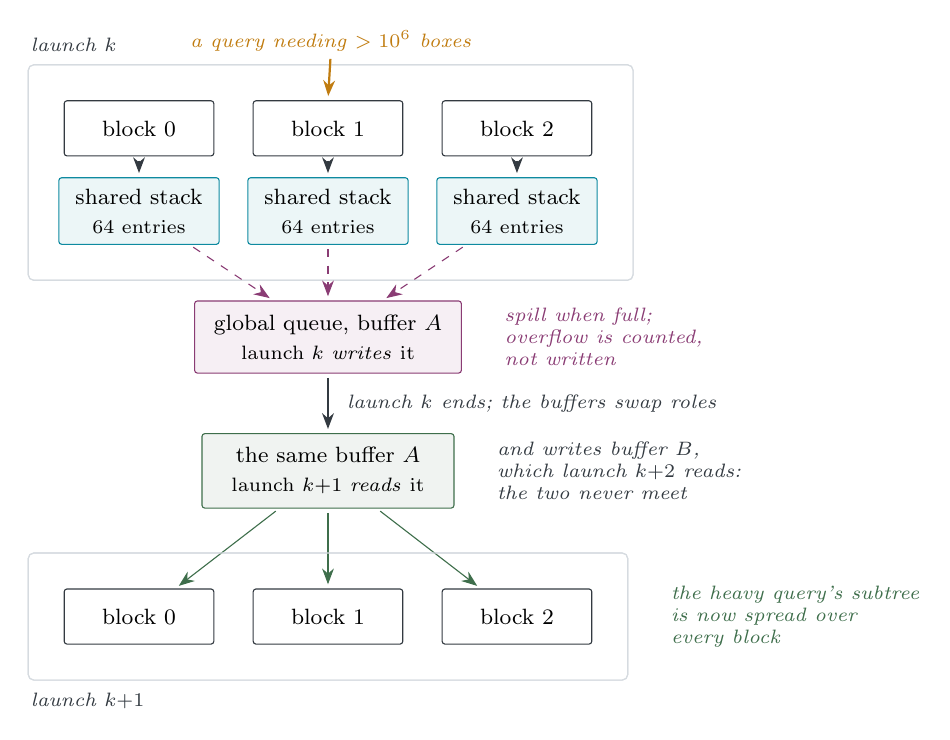
\begin{tikzpicture}[
  font=\footnotesize,
  >={Stealth[length=2mm]},
  every edge/.append style={shorten >=1.5pt, shorten <=1.5pt},
  blk/.style={draw=sccdInk, rounded corners=1pt, minimum width=19mm,
              minimum height=7mm, align=center, fill=white,
              inner xsep=6pt, inner ysep=4pt},
  stk/.style={draw=sccdTeal, fill=sccdTeal!8, rounded corners=1pt,
              minimum width=19mm, minimum height=8mm, align=center,
              inner xsep=6pt, inner ysep=4pt},
  buf/.style={draw=sccdPlum, fill=sccdPlum!8, rounded corners=1pt,
              minimum width=32mm, minimum height=9mm, align=center,
              inner xsep=7pt, inner ysep=5pt},
  lbl/.style={font=\scriptsize\itshape, text=sccdInk, align=left, inner sep=1pt},
  grp/.style={draw=sccdGrid, rounded corners=2pt, inner sep=4.5mm},
  flow/.style={->, shorten >=1.5pt, shorten <=1.5pt},
]

% ======================= launch k =======================================
\foreach \i/\x in {0/0, 1/2.4, 2/4.8} {
  \node[blk] (b\i) at (\x,1.9) {block \i};
  \node[stk] (s\i) at (\x,0.85) {shared stack\\[1pt]\scriptsize 64 entries};
  \draw[flow, draw=sccdInk] (b\i) -- (s\i);
}
\node[grp, fit=(b0)(s2)] (g1) {};
\node[lbl, anchor=south west] at ([yshift=1.2mm]g1.north west) {launch $k$};

% The pathological query arrives from outside the group.
\node[lbl, text=sccdAmber, align=center, anchor=south]
  (heavy) at ([yshift=1.2mm]g1.north) {a query needing $>10^{6}$ boxes};
\draw[flow, draw=sccdAmber, thick] (heavy.south) -- (b1.north);

% ======================= spill ==========================================
\node[buf] (wbuf) at (2.4,-0.75)
  {global queue, buffer $A$\\[1pt]\scriptsize launch $k$ \emph{writes} it};
\foreach \i in {0,1,2} {
  \draw[flow, draw=sccdPlum, dashed] (s\i) -- (wbuf);
}
\node[lbl, text=sccdPlum, anchor=west] at ([xshift=5mm]wbuf.east)
  {spill when full;\\overflow is counted,\\not written};

% ======================= swap ===========================================
\node[buf, draw=sccdMoss, fill=sccdMoss!8] (rbuf) at (2.4,-2.45)
  {the same buffer $A$\\[1pt]\scriptsize launch $k{+}1$ \emph{reads} it};
\draw[flow, draw=sccdInk, thick] (wbuf) -- (rbuf);
\node[lbl, anchor=west] at ([xshift=2mm]$(wbuf.south)!0.5!(rbuf.north)$)
  {launch $k$ ends; the buffers swap roles};

% ======================= launch k+1 =====================================
\foreach \i/\x in {0/0, 1/2.4, 2/4.8} {
  \node[blk] (c\i) at (\x,-4.3) {block \i};
  \draw[flow, draw=sccdMoss] (rbuf) -- (c\i);
}
\node[grp, fit=(c0)(c2)] (g2) {};
\node[lbl, anchor=north west] at ([yshift=-1.2mm]g2.south west)
  {launch $k{+}1$};
\node[lbl, text=sccdMoss, anchor=west] at ([xshift=5mm]g2.east)
  {the heavy query's subtree\\is now spread over\\every block};
\node[lbl, anchor=west] at ([xshift=5mm]rbuf.east)
  {and writes buffer $B$,\\which launch $k{+}2$ reads:\\the two never meet};

\begin{scope}[on background layer]
  \node[grp, fit=(b0)(s2)] {};
  \node[grp, fit=(c0)(c2)] {};
\end{scope}
\end{tikzpicture}
}
  \caption{Where a box lives in the device narrow phase. Each block keeps a
    $64$-entry stack in shared memory, visible only to its own threads, and
    spills beyond that into the half of the global queue that the current launch
    writes. The launch that follows reads that half and writes the other, so a
    producer and its consumer are never in the same launch and nothing spins. A
    subtree that crosses into the queue becomes available to every block, where
    a larger shared stack would have kept it inside the block that seeded it.}
  \label{fig:gpu-workflow}
\end{figure}

\begin{algorithm}[!tb]
\caption{Device narrow phase: a kernel that runs to completion on the work it
was given, and a host loop that relaunches it on what it spilled. $S$ is the
per-block shared stack ($64$ entries) and $G$ the double-buffered global queue.}
\label{alg:device}
\footnotesize
\begin{algorithmic}[1]
\Function{Kernel}{read buffer $G_{\mathrm{in}}$, write buffer $G_{\mathrm{out}}$}
  \State thread $t$ takes one box: its own query's root, or one entry of
         $G_{\mathrm{in}}$
  \While{any thread of the block holds a box \textbf{or} $S \ne \emptyset$}
    \State refresh the block's bound from the global minimum
      \Comment{every iteration; \cref{sec:parallel:tuning}}
    \State \textbf{if} $\dom.t_{\ell} \ge$ bound \textbf{then} idle this thread
    \If{$\mathrm{depth} \ge D$ \textbf{or} $\dom$ cannot be bisected}
      \State lower $\toi$ to $\dom.t_{\ell}$; idle this thread
        \Comment{exhaustion accepts}
    \Else
      \State $\dom.t_{h} \gets \min(\dom.t_{h},\ \mathrm{bound})$
      \State $(\dom^{-},\dom^{+}) \gets$ \Call{Split}{$\dom$}
      \State evaluate \textbf{all $8$ corners of each child}
        \Comment{all eight; \cref{alg:host} inherits four}
      \State discard a child the bound has passed or which leaves the domain
      \State \textbf{if} \Call{Accept}{} holds for a child \textbf{then} lower
             $\toi$ to its $t_{\ell}$ and discard it
      \State \textbf{if} both children remain \textbf{then} descend into the
             smaller $t_{\ell}$ and set the other aside
      \State \textbf{else if} one remains \textbf{then} descend into it
             \textbf{else} idle this thread
    \EndIf
    \If{a box was set aside}
      \State claim a slot in $S$; if $S$ is full, bump-allocate in
             $G_{\mathrm{out}}$
      \State if $G_{\mathrm{out}}$ is full, add to the deficit and
             \textbf{discard}
        \Comment{reports early, never late}
    \EndIf
    \State idle threads claim from $S$ by compare-and-swap, reloading geometry
           on a query change
  \EndWhile
\EndFunction
\Statex
\Function{Host}{candidates $\Cand$}
  \Repeat
    \State \Call{Kernel}{seeds, $A$}
      \Comment{one thread per query}
    \While{the buffer just written is non-empty}
      \State \Call{Kernel}{it, the other one}; swap the two
        \Comment{reader and writer never meet}
    \EndWhile
  \Until{the deficit is zero \textbf{or} $32$ rounds have been spent}
  \State between rounds: grow $G$ by the deficit, keeping the times of impact
         found so far
\EndFunction
\end{algorithmic}
\end{algorithm}

\subsection{Precision}
\label{sec:parallel:precision}

Both narrow phases compute in double precision internally whatever type the
caller stores geometry in, and this is a requirement of the method: in single
precision the certified bound of \cref{eq:err} and the tolerances of
\cref{eq:tol} sit too close together for the search to keep its guarantee, and
the single-precision device kernel reported nine times of impact \emph{later}
than the true root on armadillo-rollers, violating \cref{def:conservative}.

The interface stays templated on the storage type, so a caller with float
geometry keeps float buffers. Widening on load is exact, whereas narrowing the
computed time of impact back to float is not: round-to-nearest can round
\emph{up}, publishing a value later than the one the search proved, so the
narrowing rounds toward $-\infty$. Reporting earlier is always safe; reporting
later is the failure the whole design exists to prevent.

\subsection{Parameters settled by measurement}
\label{sec:parallel:tuning}

Five quantities above are constants chosen by measurement rather than by
derivation. They are collected here so that the two kernels can be read without
them, and reported because a reimplementation has to choose them too.

\emph{Vector width.} The two query types peak at different widths, since a
vertex-face corner costs one more multiply-add and one more subtraction than an
edge-edge corner and its sweeps therefore take longer to amortise the per-lane
scalar work between them. On NEON, over cloth-funnel, narrowing vertex-face from
four lanes to two moves it from $297.7$ to $246.0\,\mathrm{ms}$, and widening
edge-edge from two to four moves it from $599.9$ to $494.6\,\mathrm{ms}$; eight
and sixteen lanes are worse for both. The x86 widths quoted in
\cref{sec:parallel:host} follow from the same operation count and have not been
measured. One caveat generalises beyond this kernel: the two types must be timed
in separate processes, because timed together the edge-edge figure varies by
about $20\%$ with the lane width chosen for the \emph{vertex-face}
instantiation, which the measurement never executes. That is an effect of code
layout rather than of work, and it is large enough to manufacture or to conceal
a difference of the size reported here.

\emph{Shared-stack capacity.} Reducing the per-block capacity from $1024$
entries to $256$ and then to $64$ moves the device narrow phase from $4059.2$ to
$198.2$ and then to $37.2\,\mathrm{ms}$ on cloth-funnel, from $3133.7$ to
$277.2$ and $75.8\,\mathrm{ms}$ on armadillo-rollers, and from $129.8$ to
$110.2$ and $105.9\,\mathrm{ms}$ on cloth-ball. False positives and reported
times of impact are identical at every capacity, which is what identifies the
effect as redistribution and not pruning. The smaller stack costs nothing to hold: $3{,}584$
bytes per block against $57{,}376$ at $1024$, and the kernel is register-limited
to two blocks per multiprocessor at either capacity, so what the reduction buys
is balance and not occupancy.

\emph{Bound refresh interval.} The running minimum is re-read from global memory
on \emph{every} iteration of the device loop. Refreshing every $4$th, $16$th,
$64$th or $256$th iteration instead was monotonically worse on all three scenes
tested --- on cloth-funnel, $638.7\,\mathrm{ms}$ at every iteration against
$3377.5\,\mathrm{ms}$ at every $256$th --- because the pruning a fresh bound buys
exceeds what the atomic costs.

\emph{Unit of work per query.} One thread per query beat one block per query by
between $2.76\times$ and $4.47\times$ on the three scenes, with identical false
positives and no missed collision, because the block-per-query kernel was bound
by \emph{scheduling blocks} and not by the search: cloth-funnel issues $843{,}414$
of them, each classifying $63$ boxes across $128$ threads.

\emph{Work-list capacity.} This is the one of the five that shows up as a loss
of accuracy rather than as a slowdown, and it is worth separating because the
symptom misleads. A capacity sized from the mean is far too small for the tail. The host explores about $1.2$ boxes
per query when a shared bound is pruning and about $11$ when it is not, which
suggests a stack of a few dozen entries. On a vertex-quad query whose exact
answer is $2/3$, a $32$-entry stack reports $0.6655369599$ where $128$ and $512$
entries both report $0.6666666238$: the answer falls $1.13\times10^{-3}$ before
the true value where the triangle path reaches $3.0\times10^{-7}$. All three
values are early, so the guarantee holds throughout and only the step a solver
can take is lost --- but read as a conservativeness failure it sends an
implementer to the acceptance test, where the fault is not.

\subsection{Why the work divides the way it does}
\label{sec:parallel:why}

\Cref{tab:difficulty} counts, for every candidate pair of one scene, the boxes
each narrow phase examined before it answered. Both distributions are
heavy-tailed, which is the premise both kernels were built on: seven queries in
ten are settled by one box or none, while a few need tens of thousands and the
worst needs millions. The two differ in where the weight sits, and the
difference runs in opposite directions at the two ends of the distribution.

In total the device examines $4.8\times$ as many boxes as the host,
$106.9$ million against $22.2$, and the excess is in the \emph{middle} of the
distribution rather than in the tail: $1.33$ million device queries need at
least eight boxes against $0.82$ million host queries, and the ratio is similar
at $64$ and at $1{,}024$. A per-box factor of this kind is what
\cref{alg:host,alg:device} predict, since the device re-evaluates all eight
corners of both children at every split where the host inherits four of each
child's eight from its parent (\cref{sec:parallel:host}). That factor falls on
the operation which dominates both kernels and is paid on every box.

At the far end of the distribution the ordering reverses, and it is the host that
owns the tail. Six host queries examine more than a million boxes and its worst
examines $4{,}591{,}271$; no device query reaches a million and its worst
examines $101{,}246$, $45\times$ fewer. This is the bound schedule rather than
the search. A host block is seeded with the shared minimum as it stands when that
block starts, so a block the scheduler runs early searches a window in $t$ that
no other block has yet narrowed, and a hard query landing in such a block is
searched almost unpruned. The device issues every query of the batch in one
launch, so the minimum collapses while the hard queries are still being searched,
and spilling bounds how long any one block can be held by a single query.

Neither effect is a property of the hardware, and the second of them is the
reason the device wins the narrow phase on the scenes with the most candidate
pairs while losing it on the smallest (\cref{sec:results:proc}): the collapse of
the shared bound within a launch is worth more the more queries the launch
carries.

The broad phase inverts both arguments, having no sequential dependence and no
shared bound to lose. The GPU accordingly wins that phase on all six scenes, and
the pipeline wins end to end on four of them despite losing the narrow phase on
four. \Cref{sec:results} measures all of it.

\begin{table}[htbp]
  \centering
  \caption{Boxes examined per query on cloth-funnel, over every one of the
    $25{,}192{,}698$ candidate pairs the broad phase produced in the
    scene's $577$ steps. Both processors are handed the same
    candidates and asked for one earliest time of impact per step, so both
    prune against a shared running minimum. Each narrow phase counts its own
    boxes per query and buckets them by $\lfloor\log_{2}\rfloor$ with the same
    code, so the two columns measure the same quantity; the device's count also
    includes boxes it evaluated and then discarded because the bound had already
    passed them, which the host discards before counting, and which is
    $0.06\%$ of the device total here. Timings are not reported from this
    run: the counters serialise the device kernel.}
  \label{tab:difficulty}
  \begin{tabular}{lrr}
    \toprule
    boxes examined & host queries & device queries \\
    \midrule
    $0$--$1$                 & $18{,}852{,}925$ & $17{,}220{,}209$ \\
    $\ge 8$                  & $817{,}187$ & $1{,}332{,}867$ \\
    $\ge 64$                 & $23{,}035$ & $43{,}243$ \\
    $\ge 1{,}024$            & $2{,}046$ & $6{,}383$ \\
    $\ge 16{,}384$           & $92$ & $61$ \\
    $\ge 1{,}048{,}576$      & $6$ & $0$ \\
    \midrule
    worst single query       & $4{,}591{,}271$ & $101{,}246$ \\
    \midrule
    boxes in total           & $22{,}195{,}731$ & $106{,}911{,}080$ \\
    mean per query           & $0.88$ & $4.24$ \\
    \bottomrule
  \end{tabular}
  \par\smallskip\footnotesize Source: \texttt{benchmark/results/boxes/}
\end{table}


\section{Conservativeness by construction}
\label{sec:guarantee}

The measurements in \cref{sec:results} report no missed collision and no late
time of impact over eleven million query-mode checks. That is evidence and not a
proof, and on its own it leaves open the possibility of an untested query that
fails. This section gives the structural argument, which is short. It then says
exactly where an implementation can break that argument, which in our experience
is the part that gets used.

\begin{theorem}[Conservativeness]
\label{thm:conservative}
Suppose \cref{alg:np} is instantiated so that
\begin{enumerate}
\item[(i)] the rejection test discards a box only when the computed hull of the
  eight corner values, widened by \emph{at least} the certified bound $\epsilon$
  of \cref{eq:err}, excludes the origin on some component; a wider pad is sound,
  and the device kernels use $\max(\tau,\epsilon)$;
\item[(ii)] acceptance reports the box's lower bound in $t$; and
\item[(iii)] every terminating condition other than rejection, whether a depth
  cap, an interval the arithmetic can no longer bisect, or a full work list,
  accepts the box; and
\item[(iv)] the children produced by \op{Split} tile their parent, so every point
  of a parent lies in some child.
\end{enumerate}
Then the reported $\toi$ satisfies $\toi \le \toitrue$, and $\toi < \infty$
whenever a contact occurs.
\end{theorem}

\begin{proof}
Let $\dom$ be any box containing a root of $\Fdiff$. By \cref{eq:hull} the exact
hull of the corner values contains $\Fdiff(\dom) \ni 0$ on every component, and by
\cref{eq:err} the computed hull differs from the exact one by at most $\epsilon$
componentwise. Widening the computed hull by $\epsilon$ therefore contains the
origin, and (i) does not discard $\dom$. So no box containing a root is ever
rejected. By (iv) a box holding the earliest root has a child that also holds it,
so by induction the search retains such a box at every level it reaches.

Consider the terminal box $\dom^{\dagger}$ on that chain, the one at which the
search stops refining. By (iii) it is not dropped, so it is accepted, and by
(ii) the search reports $\dom^{\dagger}.t_{\ell}$. Since $\dom^{\dagger}$
contains the earliest root, $\dom^{\dagger}.t_{\ell} \le \toitrue$. Pruning
against the running minimum only skips boxes whose $t$ lower bound already
exceeds a value the search has attained, which by the same argument is itself
at or below $\toitrue$; so pruning cannot raise the reported value. Hence $\toi
\le \toitrue < \infty$. \end{proof}

Three consequences follow, and each is routinely stated the wrong way round.

\paragraph{Accepting is always safe, however loose the test.} Nothing in
\cref{thm:conservative} constrains \textsc{Accept}. A looser test stops refining
sooner, so it accepts an \emph{ancestor} of the box a tighter test would have
accepted. An ancestor's lower bound in $t$ is at or before its descendant's, so
the looser test reports at or earlier than the tighter one. That costs accuracy
and produces false positives. It cannot produce a late answer or a miss.
\textsc{Relaxed} and \textsc{Tight} therefore differ in accuracy and speed and
not in safety, and the two can be compared on accuracy with no safety caveat
attached.

\paragraph{A depth or stack cap is an accuracy limit, not a safety one.} By
(iii) exhaustion accepts at the box's $t$ lower bound. An undersized cap
therefore reports a time of impact earlier than the true one, and may report a
contact where none exists. It \emph{cannot} miss a collision.

The distinction matters because the effect is large enough to be mistaken for a
correctness failure. A work list sized from the average is far too small for the
tail of \cref{tab:difficulty}. The host explores about $1.2$ boxes per query when
a shared bound is pruning, and about $11$ when it is not, which suggests a
per-thread stack of a few dozen entries. On a vertex-quad query whose exact
answer is $2/3$, that choice costs four orders of magnitude of accuracy:
\begin{center}\ttfamily
\begin{tabular}{ll}
stack cap 32  & 0.6655369599 \\
stack cap 128 & 0.6666666238 \quad\rm(the host's answer)\\
stack cap 512 & 0.6666666238 \\
\end{tabular}
\end{center}
At $32$ entries the answer falls $1.13\times10^{-3}$ before the true value, where
the triangle path reaches $3.0\times10^{-7}$. Every one of the three values is
early, so the invariant holds throughout, and only the step size a solver can
take is lost. Diagnosing this as a conservativeness failure would send an
implementer to the acceptance test, which is not where the problem lives.

The remedy is to derive the capacity. Each pop pushes at
most $k$ children, so a depth-$D$ search needs $1 + kD$ entries. Sizing the work
list from the branching factor and the depth limit makes the tightness of the
answer a property of the search depth. Headroom costs almost nothing: a
$257$-entry stack is a $14.7\,\mathrm{KB}$ frame of which only the first few
entries are ever touched, and register count and spill are unchanged between
capacities $4$ and $513$.

\paragraph{The only way to lose a root is an unsound rejection.} Condition (i)
is the whole of the exposure, and it fails in exactly one way: padding the
origin-containment test by something that merely resembles the certified bound.
Two such substitutions occur in practice, and both are silent.

The first is to pad by the caller's distance tolerance $\tau$ in place of
$\epsilon$. In double precision $\epsilon$ is at most $6.7\times10^{-15}$, while
a typical tolerance is $3\times10^{-8}$. The substitution therefore changes no
answer on any realistic input, and no benchmark detects it. It leaves the search
unsound for any caller who asks for a tolerance below the error bound, and that
is the caller who most needs the guarantee to hold. Padding by
$\max(\tau,\epsilon)$ removes the dependence on what the caller passes. The
second substitution is to pad by the machine epsilon itself, which for a
bilinear query is about $30\times$ too small.

Condition (iii) admits a third failure, and it is the one that most resembles a
paradox. A depth cap that \emph{drops} an exhausted box misses a vertex falling straight
through a stationary triangle in \emph{double} precision, on a
query the same search resolves in single precision. In double the box goes on
subdividing until the cap fires, and the cap then discards it. Exhaustion has to
accept.

Taken together, the three consequences make \cref{thm:conservative} usable as a
checklist. It reduces ``is this implementation conservative'' to three local
questions, and they are the same three for whatever search is being examined.
Does the rejection test pad by the certified bound, or by something that merely
resembles it? On acceptance, is the reported value the box's $t$ lower bound?
On depth, resolution or queue exhaustion, is the box accepted and not dropped?
If all three hold, the kernel is conservative however loose or tight its
acceptance test is, and any measured violation points at one of the three and
not at the algorithm.

\section{Numerical experiments}
\label{sec:results}

This section evaluates three properties of the pipeline: conservativeness,
accuracy relative to the exact roots of the dataset, and cost on each processor.
\Cref{sec:results:cons,sec:results:ref} address the first two. The remainder of
the section reports cost, including the configurations on which the pipeline is
the slower of the two.

\subsection{Experimental setup}
\label{sec:results:setup}

All measurements are taken on the CSCS Alps system, on nodes built from the
\textsc{NVIDIA GH200} Grace Hopper superchip~\citep{nvidia2023gh200}. A node
carries four modules, each pairing a Grace host with a Hopper device over a
cache-coherent NVLink-C2C link, and every measurement here uses a \emph{single}
module, its $72$ Grace cores and its one Hopper in the same allocation, so that
a host and a device number quoted together describe one module and not a node.
Host threads are bound to that module with \texttt{numactl}, since an unbound
run spreads across all four. \Cref{tab:hardware} states the two processors.

\begin{table}[htbp]
  \centering
  \caption{The two processors of one \textsc{GH200} module, as reported by the
    operating system and the CUDA device properties on the compute nodes used.
    Peak \textsc{fp64} is derived from those clocks and the per-unit counts of
    the two architectures~\citep{arm2022neoversev2,nvidia2022hopper}; the
    bandwidth row is the best of ten \textsc{stream} triad passes.}
  \label{tab:hardware}
  \fittable{%
  \begin{tabular}{lll}
    \toprule
     & Grace (host) & Hopper (device) \\
    \midrule
    architecture & Arm Neoverse V2 & NVIDIA Hopper, sm\_90 \\
    parallel units & $72$ cores & $132$ multiprocessors \\
    maximum clock & $3.42$ GHz & $1.98$ GHz \\
    vector width & $128$-bit SVE2 & $32$-thread warp \\
    threads in flight & $72$ & $270{,}336$ \\
    L1 / shared memory & $64$ KiB per core & $228$ KiB per multiprocessor \\
    L2 cache & $1$ MiB per core & $60$ MiB \\
    L3 cache & $114$ MiB & -- \\
    memory & $119$ GiB LPDDR5X & $95$ GiB HBM3 \\
    peak \textsc{fp64} & $3.9$ TFLOP/s & $33.5$ TFLOP/s \\
    triad bandwidth & $429$ GB/s & $3{,}738$ GB/s \\
    \bottomrule
  \end{tabular}}
\end{table}

The peak \textsc{fp64} figures are the products of the unit counts and the clocks
in \cref{tab:hardware}: four $128$-bit SVE2 operations per cycle on a Neoverse
V2 core, and $64$ double-precision units on a Hopper multiprocessor. The device
therefore offers $8.5\times$ the arithmetic and $8.7\times$ the memory bandwidth
of the host, the ratio against which \cref{sec:results:proc} should be read: a
phase that does not reach it is limited by something other than the peak
figures. The measured triad reaches $93\%$ of the $4023$ GB/s the device's
$6144$-bit interface implies at $2.619$ GHz.

\subsection{Software}
\label{sec:results:software}

Everything is built with the \texttt{prgenv-gnu/24.11:v2} programming
environment at \texttt{-O3}, with \texttt{CMAKE\_CUDA\_ARCHITECTURES=90} for the
device code, and run at the default search parameters: a depth cap of $69$ and a
distance tolerance of $3\times10^{-8}$. Host loops are scheduled with
OpenMP~\citep{dagum1998openmp}; oneTBB~\citep{onetbb} is an alternative backend
and is not used here. SCCD itself has no external dependencies.

The three implementations it is measured against,
TightInclusion~\citep{wang2021tight}, Scalable CCD~\citep{belgrod2025toi} and
additive CCD~\citep{li2021codim}, are used exactly as released and built with
the same compiler and optimisation level; additive CCD is driven through oneTBB,
which follows the CPU affinity mask, so its runs are bound to one module as ours
are. Mesh input carries double-precision coordinates, so the mesh path and the
exact roots of the dataset describe the same geometry.

\subsection{Timing protocol and dataset}
\label{sec:results:protocol}

Each case is timed as three consecutive calls with separate clocks and reported
as two phases. Every table and figure uses the same four tags. \emph{BP full} is
the whole broad phase: building the swept boxes and the acceleration structure,
then querying it for overlaps. It decomposes into \emph{BP prep}, the structure,
and \emph{BP queries}, the overlap queries over it, which are the two calls the
harness times separately. The narrow phase is named by the answer requested,
since the two differ in cost: \emph{NP EToI}, for \emph{earliest time of
impact}, returns one time of impact for the whole step, so every query prunes
against the running minimum, while \emph{NP per-pair} returns one time of impact
per candidate pair and has no shared bound to prune with. Unless a table names
per-pair, its narrow-phase column is NP EToI. A figure or table that reports only
part of a phase states which part in its caption.

Device timings bracket every clock with a synchronisation, since a device phase
ends with a kernel launch that returns before the kernel completes and an
unsynchronised clock would charge the tail of a phase to whichever later call
waits for it; the competitor harness synchronises identically. The first case of
a scene is run once untimed to pay for allocation and first touch, and repeats
are separate processes, since run-to-run spread is visible only across
processes; three repeats are reported throughout, as \texttt{median / max}.

Across three repeats of a whole broad phase the spread ranges from $0.3\%$ to
$3.4\%$. That is the threshold for claiming a difference below, and margins close
to it are reported as ties.

The measurements run on the time-of-impact dataset of
\citet{belgrod2025toi,nyuccd}, six simulation scenes, three of them drawn from
the University of North Carolina Dynamic Scene Benchmark~\citep{curtis2012unc}.
Each frame is supplied both as a mesh pair and as a curated query set whose
coordinates are exact dyadic rationals and whose roots were computed
symbolically. \Cref{tab:dataset} gives the sizes; a \emph{case} is one query
type on one frame, so a simulation step is two cases.

\begin{table}[htbp]
  \centering
  \caption{The benchmark problems. \emph{cases} is simulation steps with a runnable query set, \emph{candidate pairs} the mean number the broad phase produces per step, and \emph{queries} the curated per-step query sets that carry exact symbolic roots.}
  \label{tab:dataset}
  \fittable{%
\begin{tabular}{lrrrr}
    \toprule
    scene & cases & pairs/step & queries & w/ root \\
    \midrule
    armadillo-rollers & 781 & 109,214 & 131,441 & 130,859 \\
    cloth-ball & 79 & 2,217,099 & 664,940 & 664,919 \\
    cloth-funnel & 577 & 43,661 & 7,552 & 6,773 \\
    n-body & 146 & 15,436,757 & 2,947,719 & 2,947,611 \\
    puffer-ball & 240 & 30,529,227 & 1,514,172 & 1,486,790 \\
    rod-twist & 4,571 & 847,250 & 549,208 & 285,431 \\
    \bottomrule
  \end{tabular}}
  \par\smallskip\footnotesize Source: \texttt{benchmark/results/sweep-gh200-bp.csv}
\end{table}


\subsection{Conservativeness}
\label{sec:results:cons}

\Cref{tab:conservativeness} compares every query carrying an exact root against
that root, signed, on both processors and all six scenes. Summing the table,
$5{,}815{,}032$ queries carry ground-truth data and are checked on each of two
processors, giving $11{,}630{,}064$ query-mode checks. Of these,
$11{,}044{,}766$ place a reported time of impact beside an exact root and do not
merely agree that none exists. No collision is missed, and no time of impact is
reported after the true one.

\begin{table}[htbp]
  \centering
  \caption{Conservativeness against the dataset's exact roots. \emph{late} counts queries whose reported time of impact falls after the true one; it must be zero, because a late time of impact lets a simulation step through the contact, which is the failure the search exists to prevent. False positives cost work only and are reported for information. \emph{queries} is how many carry ground-truth data at all, no-collision cases included; \emph{toi compared} is how many times of impact were actually placed beside an exact root, which is what the claim rests on.}
  \label{tab:conservativeness}
  \fittable{%
\begin{tabular}{llrrrrr}
    \toprule
    scene & mode & queries & toi compared & late & false pos. & false neg. \\
    \midrule
    armadillo-rollers & GPU & 131,441 & 130,859 & 0 & 24 & 0 \\
    armadillo-rollers & CPU & 131,441 & 130,859 & 0 & 24 & 0 \\
    cloth-ball & GPU & 664,940 & 664,919 & 0 & 1 & 0 \\
    cloth-ball & CPU & 664,940 & 664,919 & 0 & 1 & 0 \\
    cloth-funnel & GPU & 7,552 & 6,773 & 0 & 15 & 0 \\
    cloth-funnel & CPU & 7,552 & 6,773 & 0 & 15 & 0 \\
    n-body & GPU & 2,947,719 & 2,947,611 & 0 & 12 & 0 \\
    n-body & CPU & 2,947,719 & 2,947,611 & 0 & 11 & 0 \\
    puffer-ball & GPU & 1,514,172 & 1,486,790 & 0 & 558 & 0 \\
    puffer-ball & CPU & 1,514,172 & 1,486,790 & 0 & 536 & 0 \\
    rod-twist & GPU & 549,208 & 285,431 & 0 & 1,245 & 0 \\
    rod-twist & CPU & 549,208 & 285,431 & 0 & 1,243 & 0 \\
    \bottomrule
  \end{tabular}}
  \par\smallskip\footnotesize Measured against the exact roots shipped with the dataset, not against TightInclusion: TightInclusion's own answer is itself a lower bound on the truth, so comparing against it over-reports lateness.
  \par\smallskip\footnotesize Source: \texttt{benchmark/results/sweep-gh200-bp.csv}
\end{table}


The comparison is made against the exact roots of the dataset and not against
TightInclusion, whose own answer is a conservative lower bound on the truth:
scoring lateness against the reference would count as a violation every case in
which our search lands closer to the root than the reference does. False
positives range from $1$ on cloth-ball to $1{,}245$ on rod-twist; they cost work
and never safety (\cref{sec:np}), and we report them as the price of the
guarantee.

\subsection{Against TightInclusion}
\label{sec:results:ref}

TightInclusion computes the same quantity by the same mathematics, so it is the
one comparison in this paper that can be made answer by answer rather than only
in aggregate. Two questions are asked of it. Does SCCD return what the reference
returns, given that \cref{prop:order} predicts it should? And what does the
reorganised search cost?

The protocol follows from the first question. TightInclusion ships no broad phase
that we use, so the comparison is of narrow phases alone and both sides are
handed the same curated query sets, at the same depth cap and the same distance
tolerance. Both are asked for one time of impact per candidate pair, since
TightInclusion maintains no bound across queries and giving it one would compare
two different computations. It is run depth-first, its faster configuration when
there is no bound to exploit, and both sides are scheduled through the same
dynamic parallel loop. TightInclusion runs on the host, so in
\cref{fig:reference} the CPU bar is the like-for-like comparison and the GPU bar
reports what the same search costs once it is moved to the other processor.

On the first question the agreement is exact where \cref{prop:order} says it
should be. Both processors reproduce the reference's hit count on every scene. To
compare the \emph{values} we report \emph{earliness}: every answer from either
implementation is a lower bound on the true root, so the quantity of interest is
how far before that root each one lands, measured against the dataset's exact
symbolic roots and summarised per scene and query type --- twelve scene-phases
--- as a median over cases and as the worst case anywhere in the scene. On the
host both statistics are identical to TightInclusion's on all twelve, to every
printed digit. That is the empirical counterpart of \cref{prop:order}: the host
kernel generates the same accepted set and therefore the same minimum, however
differently it walks the tree.

The device agrees closely without agreeing exactly, which the same proposition
anticipates. Its median matches on eight of the twelve scene-phases and its worst
case on nine, with every deviation at most $0.65\%$ on the median and $4.5\%$ on
the worst case, in both directions and smaller than the spread between repeats.
The traversal order does not explain this, by \cref{prop:order}, and no shared
minimum exists for threads to race over here, since the comparison is per pair.
The explanation is that the device evaluates the same formulas through a
different and equally valid sequence of floating-point operations --- vector
fused multiply-adds for the corner values, and for $\delta^{3}$ in \cref{eq:err}
a plain cube scaled to round upward --- so the two kernels accept slightly
different sets of boxes, and a box whose classification turns on the last few
units in the last place can fall either way. Both sequences stay inside the
certified bound, so both remain conservative; where the device additionally
discards work under queue pressure (\cref{sec:parallel:device}) the effect is
one-sided by construction. Every earliness measured, on either processor, is at
or before the exact root.

On the second question, cost, SCCD is between $2.1\times$ and $3.5\times$ faster
than the reference on the host, and the device widens that to between
$2.6\times$ and $20.9\times$. Rod-twist is the extreme case in both directions:
the reference is slowest there in absolute terms, $507.8\,\mathrm{s}$ against our
host's $221.3$, and the device gains most, finishing in $24.3$. Cloth-funnel is
the one scene on which the device does not help, its two bars standing level.

\begin{figure}[htbp]
  \centering
  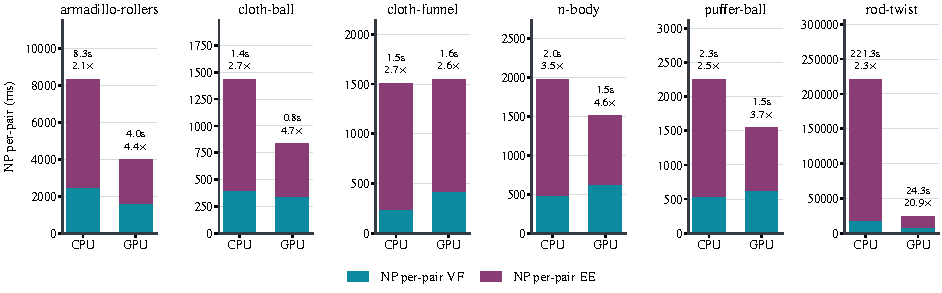
\includegraphics[width=\linewidth]{figures/reference-speedup.pdf}
  \caption{The narrow phase against TightInclusion, per scene, as whole-scene
    totals. Neither side runs a broad phase, so both are handed the same curated
    query sets and asked for one time of impact per candidate pair. Each bar is
    one processor, stacked into its vertex-face and edge-edge work, with the
    total and the speedup above it. Query counts are in \cref{tab:dataset} and
    hit agreement in \cref{tab:conservativeness}.}
  \label{fig:reference}
\end{figure}

The worst cases are a property of the problem. On cloth-funnel and rod-twist the
largest error approaches $1.0$ for the reference as well: a conservative search
has no tighter answer available on a grazing or already-touching configuration,
since the root box cannot be refined away when the contact occurs at the start
of the step.

\subsection{CPU against GPU}
\label{sec:results:proc}

\begin{table}[htbp]
  \centering
  \caption{Host against device for the same mode and the same cases. Every time is a whole-scene total in milliseconds, summed over every case of the scene. \emph{BP full} is the whole broad phase, the acceleration structure plus the queries over it; \emph{BP prep} is the structure alone and \emph{BP queries} the queries alone; \emph{NP} is the narrow phase. \emph{total} is BP full + NP, median over repeats. A ratio above one means the GPU is faster.}
  \label{tab:processor}
  \fittable{%
\begin{tabular}{lrrrrr}
    \toprule
    scene & CPU ms & GPU ms & total$\times$ & BP full$\times$ & NP$\times$ \\
    \midrule
    armadillo-rollers & 3,335 & 4,790 & 0.70x & 0.81x & 0.46x \\
    cloth-ball & 2,356 & 1,240 & 1.90x & 1.64x & 3.40x \\
    cloth-funnel & 2,073 & 3,892 & 0.53x & 0.56x & 0.41x \\
    n-body & 17,319 & 7,398 & 2.34x & 1.67x & 12.13x \\
    puffer-ball & 99,117 & 28,257 & 3.51x & 2.90x & 15.14x \\
    rod-twist & 75,502 & 37,829 & 2.00x & 2.02x & 1.97x \\
    \bottomrule
  \end{tabular}}
  \par\smallskip\footnotesize A ratio is the host median over the device median, so 2.0 means the device takes half the time. Ratios below 1.0 are the cases where the host wins and are the ones worth reading.
  \par\smallskip\footnotesize Source: \texttt{benchmark/results/sweep-gh200-bp.csv}
\end{table}


\Cref{tab:processor} reports the two processors as whole-scene totals, and the
split follows \cref{sec:parallel:why}. The broad phase is count, prefix sum and
scatter, and it runs between $0.45\times$ and $2.45\times$ of host speed. The
narrow phase is a divergent depth-first search and spans a far wider range,
$0.49\times$ to $16.51\times$: behind the host where the candidate lists are
smallest, and ahead by an order of magnitude on n-body and puffer-ball, where
billions of candidates keep every lane busy. The device's margin rests on the
narrow phase, and the broad phase decides how much of it survives.

End to end the two effects cancel to different degrees. The device wins
cloth-ball by $2.37\times$, rod-twist by $2.06\times$, n-body by $2.05\times$
and puffer-ball by $1.88\times$; the host wins armadillo-rollers at $0.95\times$
and cloth-funnel at $0.96\times$, both within five per cent of parity. On
cloth-funnel the device's broad phase is ahead at $1.29\times$ and its narrow
phase behind at $0.64\times$, so the narrow phase alone carries that scene's
gap. The two scenes the host takes are the two smallest by candidate pairs,
$25.2$ and $85.3$ million, and the device takes every scene from $175$ million
upwards. Above that the margin falls as the problem grows, cloth-ball at $175$
million pairs giving $2.37\times$ where puffer-ball at $7.33$ billion gives
$1.88\times$, so problem size indicates the processor without setting the
margin. \Cref{sec:results:scaling} varies it directly.

\Supp{} states the same comparison as a rate and per simulation step, and plots
the per-step cost through each scene. Two observations there qualify the
medians: on cloth-funnel the device is behind on $82\%$ of the frames, so its
$0.96\times$ is a standing gap and not a few expensive frames, and on rod-twist
the cost climbs steadily on both processors as the rod winds up, so the median
understates the end of the simulation.

\Cref{fig:breakdown} splits the same runs by phase: the broad phase takes $19$
to $65\%$ of the host total on every scene and $24$ to $93\%$ on the device, and
within the host's broad phase the structure it builds is the part that scales
worst with thread count (\cref{sec:results:threads}). Behind those medians,
broad-phase time is tight around its own median while narrow-phase time is
skewed by a long upper tail, the per-case form of the heavy-tailed difficulty of
\cref{tab:difficulty}; \supp{} gives the distributions. \Cref{fig:toierr} gives
the earliness distribution, one-sided by construction since every value is the
distance \emph{before} the true root at which the answer falls, with additive
CCD on the same cases beneath it.

\begin{figure}[htbp]
  \centering
  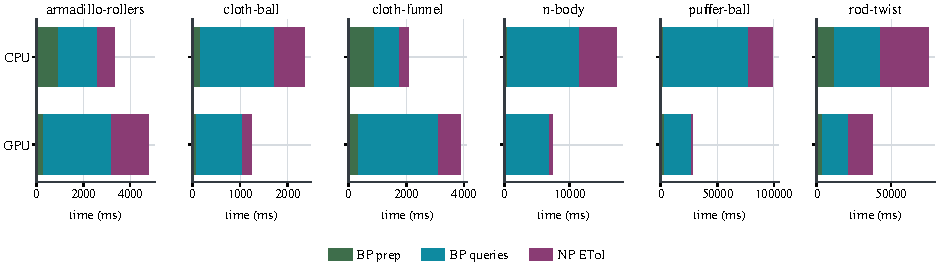
\includegraphics[width=\linewidth]{figures/runtime-breakdown.pdf}
  \caption{Whole-scene totals split into BP full and NP EToI, as a share of each
    processor's total. The BP bar is shaded into BP prep, the structure it
    builds, and BP queries over it. BP full dominates on the host, and within it
    BP prep.}
  \label{fig:breakdown}
\end{figure}

\begin{figure}[htbp]
  \centering
  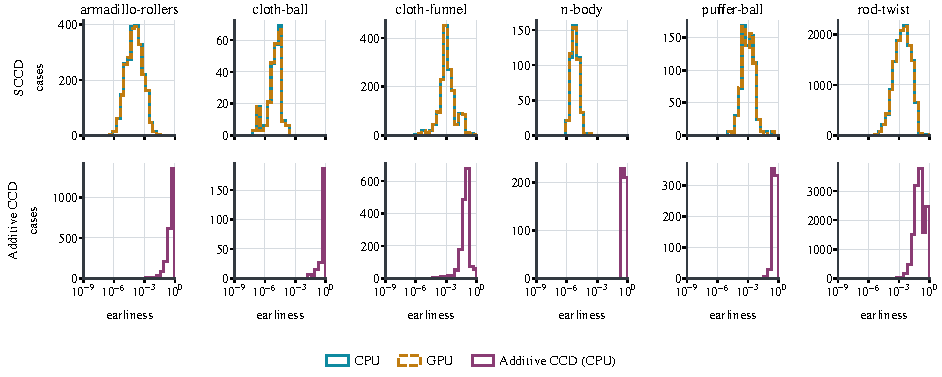
\includegraphics[width=\linewidth]{figures/earliness.pdf}
  \caption{Earliness against the exact symbolic roots, logarithmic axis, one
    value per case: the largest earliness anywhere in that case. Above, SCCD on
    both processors; below, additive CCD on the same cases, from the one
    comparison run of \cref{sec:results:others} and in the same bins. Every
    reported time of impact lies at or before its root, so both distributions
    sit on the early side of zero and nothing falls outside the axis on the late
    side. Additive CCD's
    median case sits between $1.6$ and $4.8$ decades further from the root,
    depending on the scene.}
  \label{fig:toierr}
\end{figure}

\subsection{Against other implementations}
\label{sec:results:others}

Two further implementations answer neighbouring questions, and each is compared
on the question it answers: Scalable CCD~\citep{belgrod2025toi} returns one
earliest time of impact for a simulation step, and additive
CCD~\citep{li2021codim} returns one per pair. Both are used exactly as released,
built with the same compiler flags, and run on the same node over all six scenes
and all $6{,}394$ cases, three repeats each, over identical broad-phase
candidates. \Cref{fig:competitors} summarises both comparisons per scene;
\supp{} carries the per-scene tables with their accuracy columns.

\begin{figure}[htbp]
  \centering
  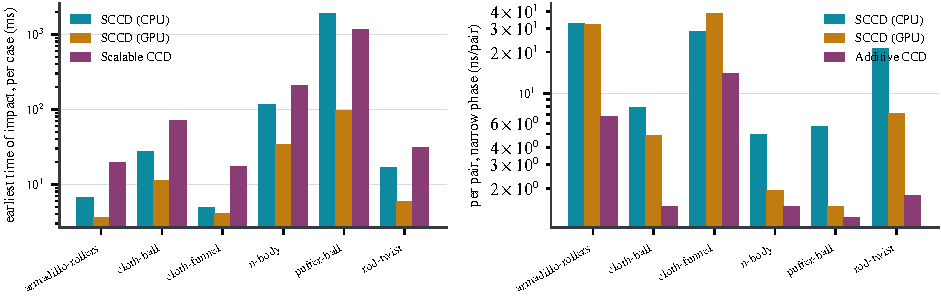
\includegraphics[width=\linewidth]{figures/competitors.pdf}
  \caption{SCCD against the two implementations that answer neighbouring
    questions, each on the question it answers. \textbf{Left}, the earliest time
    of impact for a simulation step against Scalable CCD, as the mean cost of one
    case on a logarithmic axis. \textbf{Right}, one time of impact per candidate
    pair against additive CCD, in nanoseconds per candidate.}
  \label{fig:competitors}
\end{figure}

Against Scalable CCD, SCCD on the device is ahead end to end on every scene,
from $4.23\times$ on cloth-funnel to $11.93\times$ on puffer-ball: $27.0$
against $142.9\,\mathrm{s}$ over rod-twist's $4{,}571$ cases, and $23.3$ against
$278.3\,\mathrm{s}$ over puffer-ball's $240$. Puffer-ball is also the scene on
which our host path loses outright, at $458.6\,\mathrm{s}$, since its broad
phase carries the scene on its own. The comparison is on the device throughout,
because the narrow phase of Scalable CCD is CUDA and its host side is a broad
phase with no pipeline behind it.

\Cref{fig:bpvs} compares the two broad phases step by step. Summed over the
benchmark ours costs $40.3\,\mathrm{s}$ against $312.6\,\mathrm{s}$, and the
margin is a standing one: on puffer-ball, the scene with the most candidate
pairs, it is $21.9\,\mathrm{s}$ against $226.8$. Drawing both of our strategies
separates what the implementation earns from what the choice of algorithm earns.
On n-body the two differ, our sweep being the slower broad phase there,
$7.5\,\mathrm{s}$ against Scalable CCD's $6.3$, while our cell list takes the
scene at $4.5$; on cloth-funnel the two are within $18\%$ of each other and both
far ahead, so the $5.4\times$ against Scalable CCD is attributable to the
implementation.

\begin{figure}[htbp]
  \centering
  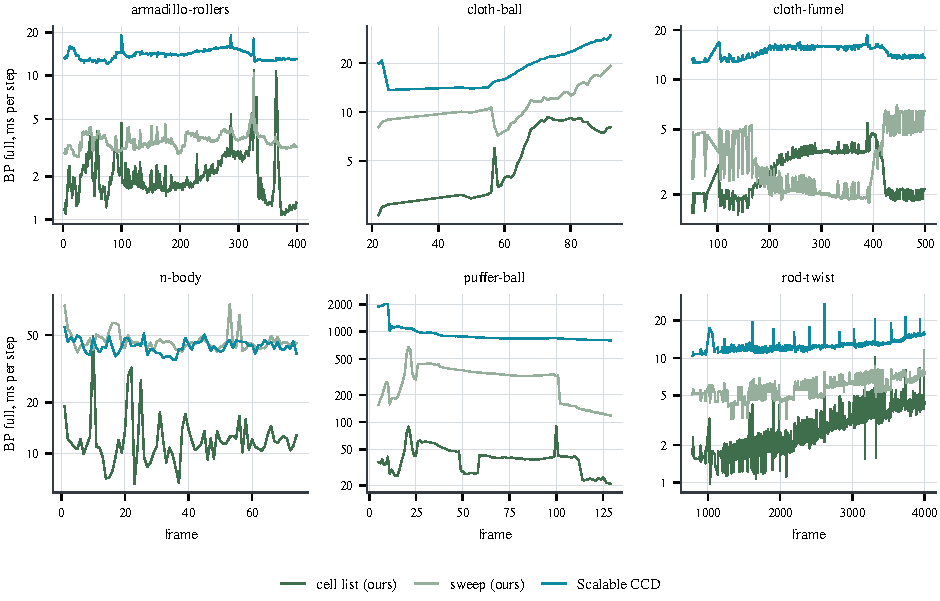
\includegraphics[width=\linewidth]{figures/broad-vs-scalable.pdf}
  \caption{Device BP full against Scalable CCD's, step by step, the
    acceleration structure and the queries over it added, in milliseconds for
    one step, both query types together. All three curves come from one
    comparison run, so they are measured in one allocation. Both of our
    strategies are drawn, since the choice between them accounts for part
    of the difference.}
  \label{fig:bpvs}
\end{figure}

Its earliness columns report a defect on three scenes and not a difference in
tightness: its answer lands after the true root on $269$ of armadillo-rollers'
$394$ contact-carrying steps, $31$ of rod-twist's $2{,}481$ and $9$ of
cloth-funnel's $363$. We traced this to a race in its subdivision buffer, whose
overflow check tests that the buffer is full and then advances the tail as two
separate operations; \supp{} gives the three observations that identify it. We
report the library as published. Where it does stay conservative it remains the
looser answer, against our device by $50.7\times$ on cloth-ball, $281\times$ on
rod-twist and $2{,}844\times$ on puffer-ball.

Additive CCD advances conservatively until contact without isolating a root, and
it is the cheaper narrow phase per candidate: by $7.1\times$ on rod-twist,
$4.9\times$ on armadillo-rollers, $2.7\times$ on cloth-funnel and $2.3\times$ on
cloth-ball, against our narrow phase on the host. The margin closes as the problem
grows, and on the two scenes carrying the most candidate pairs the two meet, at
$1.0\times$ on n-body and $1.1\times$ on puffer-ball, where billions of
candidates keep every lane of the host busy.

The cost of that speed is the answer. Its median earliness runs from
$2.3\times10^{-2}$ to $1.1\times10^{-1}$ where ours runs from
$3.0\times10^{-8}$ to $3.2\times10^{-4}$, which \cref{fig:toierr} shows as a
separation of between $1.9$ and $6.3$ decades, and its worst case gives up almost
the entire step on every scene, between $0.897$ and $0.996$. The false positives
follow: $444$ against $24$ on armadillo-rollers and $27{,}374$ against $536$ on
puffer-ball. Neither library misses a contact anywhere and neither
answers after a root, which for both follows from the construction of the method
rather than from the measurement. A solver pays for the gap with a shortened step.

\subsection{Scaling with element count}
\label{sec:results:scaling}

The refinement study reported in \supp{} refines one surface repeatedly,
quadrupling the element count at each level from $92{,}230$ to $94.4$ million
over cloth-ball frames $0$ and $1$. Both processors run the shipped broad phase,
so the one quantity it varies is the processor, and the two frames do not come
into contact, which makes the broad phase the quantity it measures.

\begin{figure}[htbp]
  \centering
  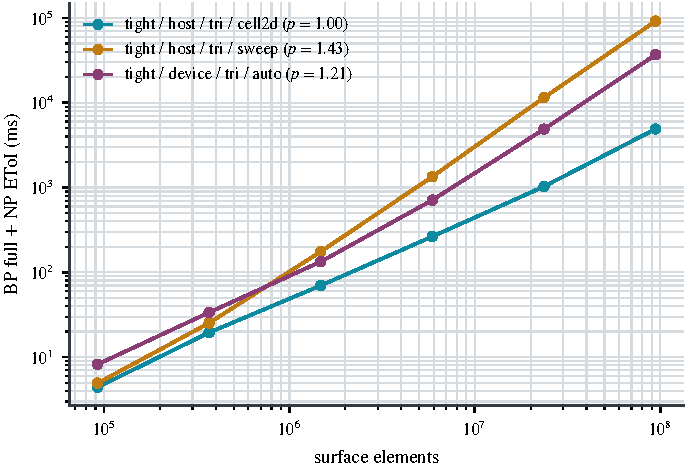
\includegraphics[width=0.62\linewidth]{figures/refine-scaling.pdf}
  \caption{Cost of one collision step against element count, log--log. Each
    series is one processor, and $p$ is the exponent fitted to the plotted
    quantity, BP full plus NP EToI.}
  \label{fig:scaling}
\end{figure}

\Cref{fig:scaling} plots both processors on logarithmic axes; they cross between
$5.90$ and $23.6$ million elements, and the device leads above that size. Taking
the whole broad phase, the host is ahead through the middle of the range by at
most $1.29\times$ ($51.6\,\mathrm{ms}$ against $66.7$ at $1.48$ million), and its
margin has already closed to $1.07\times$ at $5.90$ million ($243.7$ against
$260.7$). Past the crossing the device pulls away: $2.34\times$ at $23.6$ million
($343.5$ against $802.9$) and $2.58\times$ at $94.4$ million ($1472.5$ against
$3801.9$). The fitted exponents place the device at $0.80$ in the element count
and the host at $1.03$.

The two halves of the broad phase divide differently by processor. At $94.4$
million elements the structure costs $50.4\,\mathrm{ms}$ on the device and
$808.9$ on the host, a factor of $16.0$, while the queries over it take
$1422.2\,\mathrm{ms}$ against $2993.0$, a factor of $2.10$. The structure is
therefore $3.4\%$ of the device's broad phase and $21.3\%$ of the host's: binning
is a counting sort, the histogram is a reduction over the element count, and both
are shapes the device answers at full width. The queries carry the remainder, and
their smaller factor is what sets the device's slope.

The narrow-phase column measures a different quantity, since no root is ever
isolated on these two frames and it therefore prices the rejection test alone
over candidates that all fail it. That work is uniform, the shape a GPU handles
best: the device stays between $2.7$ and $9.2\,\mathrm{ms}$ across the six
refinements while the host climbs from $0.3$ to $130.8$, ending $14.2\times$
ahead on a column where it began $10.0\times$ behind. It is silent on the
divergent case, for which \supp{} gives narrow-phase cost against problem
size.

\subsection{Scaling with thread count}
\label{sec:results:threads}

\Cref{sec:results:scaling} varies the problem and holds the machine fixed.
Holding the problem fixed instead and varying the thread count from one to
seventy-two Grace cores separates the phases of the host pipeline
(\cref{fig:strong}).

Two of the three scale well. The overlap queries reach $32.0\times$ and the
narrow phase $40.4\times$ at seventy-two cores, which is what \cref{alg:host} is
built for: lanes are filled from a work list private to a block, blocks are
independent, and the only shared state is an atomic minimum written rarely.

Building the acceleration structure is the limit. It reaches $5.9\times$ at
thirty-two cores and goes no further, so a pass taking $8$ to $13\%$ of the
single-core time takes $38$ to $48\%$ of it at seventy-two and holds the whole
pipeline to between $13.2\times$ and $24.0\times$. Three passes over every box
account for the plateau, all of them reductions or histograms: the
centre-variance reduction that picks the two grid axes, the extent and mean
reduction that sizes the grid, and the counting histogram that fills it. What
remains once those are parallel is a fixed cost per call rather than a share of
the work, which is why further cores cannot recover it --- between sixty-four and
seventy-two cores every curve is flat, so none of the figures quoted here depends
on which of the two counts it is read at.

\begin{figure}[htbp]
  \centering
  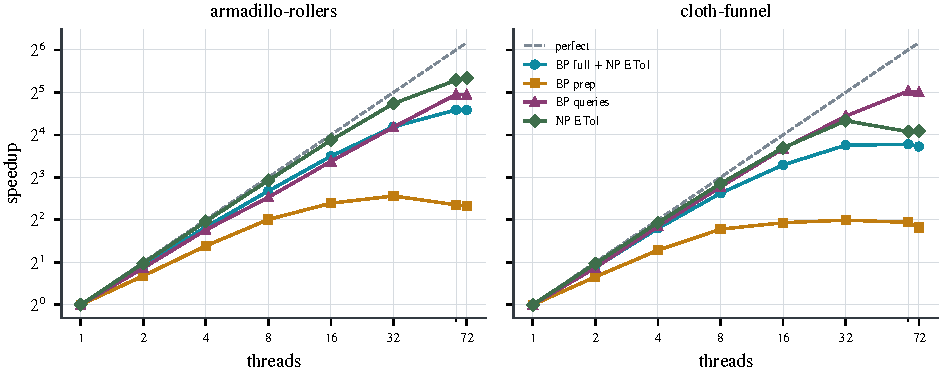
\includegraphics[width=\linewidth]{figures/strong-scaling.pdf}
  \caption{Strong scaling of the host pipeline by phase, as whole-scene totals
    against the perfect line. The narrow phase tracks it closely; the structure
    the broad phase builds leaves it early and plateaus around thirty-two cores.}
  \label{fig:strong}
\end{figure}

\section{Limitations and threats to validity}
\label{sec:limitations}

Every figure in \cref{sec:results} is checked against exact roots by a gate that
fails on a missed collision or a late time of impact, and the data behind each
table is published alongside the code. Three kinds of limitation nevertheless
lie outside what those numbers establish: the reach of the ground truth they are
measured against, the reach of the measurement itself, and the parts of the
pipeline that carry no measurement.

\subsection{What the ground truth reaches}

The dataset ships symbolic roots for its curated \emph{query sets} and not for
the mesh frames, so everything in \cref{sec:results:cons,sec:results:ref} is
measured on the query sets. The mesh path is checked only for
\emph{agreement}: the answer computed over the mesh is compared against the
earliest exact root of the corresponding query set, and a disagreement would
mean the two paths were handed different geometry. This is a tripwire on the
inputs, not a verification of the kernel.

The two paths do differ in the geometry they carry. The mesh container stores
coordinates in single precision, and armadillo-rollers needs $52$ significand
bits to represent its dyadic rationals exactly. The resulting divergence between
mesh and query geometry is two-sided, and it ranges from $5\times10^{-8}$ to
$4.6\times10^{-5}$. An accuracy claim tighter than that, made on the mesh path,
measures the rounding and not the search.

Deliberately inflicting that rounding shows the size of its effect. On the same
$98{,}757$ armadillo-rollers edge-edge queries, \textsc{Tight} reports no missed
collision and no late time of impact on the shipped double-precision geometry.
Once the input is first rounded through single precision, it reports $4$ missed
and $25{,}485$ late. A control settles where the fault lies: a host kernel
bit-identical to TightInclusion, already computing in double, reports zero late
on the shipped geometry and $4{,}543$ late under the same treatment. The cause
is the input rounding and not either kernel. Single-precision-geometry runs are
therefore reported separately and never gate the build, and the comparison is
the empirical form of the argument in \cref{sec:parallel:precision}.
\textsc{Tight} is hurt about fourteen times more than \textsc{Relaxed} here
\emph{because} it reports closer to the true root: a perturbed root crosses a
tight answer far more often than it crosses a loose one.

\subsection{What a measurement establishes}

When the caller asks only for the earliest time of impact, workers prune against
a shared atomic minimum, so the exact value depends on the order in which they
publish. Every value observed is at or before the true root, and the guarantee
is unaffected. The last digits do move between runs, however, so a test that
pins a time of impact to better than about $10^{-6}$ will be flaky. The same
applies to the quad path.

Non-determinism of that kind can also hide a defect. During this evaluation one
repeat of one scene showed the device \textsc{Relaxed} kernel missing $2$
collisions and reporting $5$ late of $15{,}957$ queries. The next repeat over
identical input was clean, as were the other five scenes and the other three
modes across the remaining $65{,}079{,}040$ checks of that run. The cause was a
single index, which pruned the root box against the first query's answer in
place of its own. This occurs only when the first query reports exactly zero, so
whether a collision was missed depended on block scheduling. Twelve repeats of
the case failed five times before the fix and none after it, and every device
figure in this paper is taken after the fix.

The episode bounds what a check can establish, not what the kernel does. A
defect surfacing in about two runs in five is invisible to a spot check and
survives a benchmark that reports only agreement; separating it from noise takes
a signed comparison against exact roots, run over every query and repeated.

A last caveat concerns the timings, not the answers. The driver does more per
case than the pipeline does: it loads the frame, classifies every candidate pair
against the expected set, and compares every answer against an exact root. A
case costs between $0.7$ and $3.3\,\mathrm{s}$ of wall clock across the six
scenes, against measured work of a few tens of milliseconds. The timers exclude
all of it, so the figures are sound as timings, although the harness remains no
model of what the pipeline costs inside a solver.

\subsection{What was not measured}

Three parts of the pipeline carry no measurement here, and each bounds a claim
made earlier.

Ordering each cell's entries on the axis the grid does not use is implemented
on the host only, where it is measured and does not pay
(\cref{sec:bp:self}); the device therefore carries no such kernel and the
question is open on that processor.

The quad path is described in \cref{sec:np:quad} and evaluated nowhere. Every
scene in this benchmark is a triangle mesh, and the error constant of
\cref{sec:prelim:err} for the bilinear form is uncertified. What is established
for that path is correctness against a densely sampled reference root, and
nothing about its speed or its accuracy at scale.

Most consequentially, the closest prior work is cited and not measured against.
\citet{belgrod2025toi} evaluate a GPU CCD pipeline on these six scenes against
this ground truth, and theirs, not TightInclusion, is the state of the art in
\emph{parallel} CCD. TightInclusion answers the question this paper puts first,
which is whether the answer is right and how close it falls to the exact root,
and it answers that as a certified reference running unmodified on the same
hardware. The remaining question, whether this parallel design is faster than
that parallel design, is left open. Settling it requires building that pipeline
on \textsc{GH200}, matching the two on tolerance, depth cap and output mode so
the searches do comparable work, and timing both inside one allocation. Until
then the speedups of \cref{sec:results:ref} are margins over a host reference
and not over prior parallel work.

The counter measurements of \cref{sec:parallel:limits} are narrower than the
timings they explain. They cover all six scenes, but only one narrow-phase mode
and only the earliest-impact kernel. The device figures are taken under a
profiler that serialises launches, so they support statements about ratios and
none about absolute time. The Grace rows are whole-process counters and not
per-phase ones. The pipeline row comes from a build with the device path
compiled out, so it is host work throughout. The narrow-phase row comes from the
oracle, which also drives the device modes, so its instruction rate is a floor
and not an estimate. These counters establish which resource each processor is
short of, a coarser claim than a per-phase model would make.

Beyond the pipeline itself, three things are absent. There is no
minimum-separation CCD, which solvers in the barrier family generally want, and
no multi-GPU execution. Nor is there any measurement inside a solver, so the
end-to-end benefit of the speedups reported here is inferred and not
established.

\section{Software and data availability}
\label{sec:availability}

SCCD is released under the BSD 3-Clause licence~\citep{sccd}. The library builds
and its tests run with no external dependencies, no network access and no
configuration:

\begin{quote}
\begin{verbatim}
cmake -S . -B build && cmake --build build -j
ctest --test-dir build
\end{verbatim}
\end{quote}

\noindent
The device kernels, the smesh mesh interface and the TightInclusion accuracy
oracle are opt-in CMake options; the oracle is a validation tool and not a
performance option.

Every table and figure in \cref{sec:results} is generated from a published
measurement file by a published script. The table sources of this article come
from the same code that produces the software's own benchmark reports, so each
figure has a single origin. The regeneration command is recorded next to the
tables, and a \verb|--check| mode re-derives the documents from the data and
returns non-zero if they no longer match.

The counters of \cref{sec:parallel:limits} are collected by
\texttt{benchmark/scripts/profile.sbatch.sh}, one job that runs Nsight Compute
over the device search kernel and \texttt{perf stat} over the host. Their raw
output is published under \texttt{benchmark/results/profile/}, and
\cref{tab:counters} is generated from those files by a script in the article's
own directory, so no counter in it is transcribed by hand. Profiling changes no
result and gates nothing.

The benchmark scenes, the curated query sets and the exact symbolic roots are the
time-of-impact dataset of \citet{belgrod2025toi}, obtained from the NYU Faculty
Digital Archive~\citep{nyuccd}. We are grateful to its authors for producing
ground truth at this scale, without which none of the accuracy claims in this
paper could be made. TightInclusion~\citep{wang2021tight}, as distributed in the
IPC Toolkit~\citep{ipctoolkit}, is used exactly as released and is never
modified. Fairness in the comparison of \cref{sec:results:ref} is bought by
changing our harness to match its configuration, never the other way round.

\section{Conclusion}
\label{sec:conclusion}

We have presented a continuous collision detection pipeline whose answer is
conservative by construction on two very different processors, and measured it
against a certified reference on a dataset with exact roots. The accuracy
result is the one to take away. On the host, the median and worst-case error
match TightInclusion's on all twelve scene-phases to every printed digit, at
between $1.7\times$ and $4.9\times$ its speed. That reproduces the reference exactly. On the device, faster again by $2.5\times$ to
$26.6\times$, the two agree to within a few percent.

The design results generalise beyond this problem. \Cref{prop:order} is the
useful one. A branch-and-bound search becomes order-independent once it keeps a minimum over
all accepted leaves, in place of returning the first leaf a priority queue hands
it. Order-independence then allows vector lanes and thread
blocks to be filled with work from unrelated queries. Both of our parallel
kernels are consequences of that observation, spent in opposite directions:
packing lanes across queries on the host, and pushing work out of the block
that generated it on the device.

Two negative results carry as much as the positive ones. Four cheap statistics
that ought to predict which broad phase is faster all fail on real geometry,
and so does fixing the choice. The two algorithms rank oppositely depending on
whether one times the traversal or the whole phase, and they change places
again with the thread count. Measuring on two consecutive steps is cheaper and
more reliable than any of it. The second negative result is that a principled
splitter, aimed at the largest root-free region, loses to a crude clamped one.
A branch-and-bound search cannot exploit dead volume as such. It can exploit
only volume that a \emph{single} component rules out, and a multi-way split
lets different children die by different components.

Three next steps are obvious. Minimum-separation queries are generally required
by the barrier-method solvers this work targets. Multi-GPU execution is a
natural fit for the double-buffered queue, which already has the right shape
for it. An in-solver evaluation is the one that matters most: without it, the
practical value of these speedups stays inferred and unmeasured.


\bibliographystyle{plainnat}
\bibliography{refs}

\end{document}
